\documentclass[output=paper
                ,modfonts
                ,nonflat
	        ,collection
	        ,collectionchapter
	        ,collectiontoclongg
 	        ,biblatex
                ,babelshorthands
                ,newtxmath
                ,draftmode
                ,colorlinks, citecolor=brown
] {langscibook}

\IfFileExists{../localcommands.tex} {%hack to check whether this is being compiled as part of a collection or standalone
  % add all extra packages you need to load to this file 

\usepackage{graphicx}
\usepackage{tabularx}
\usepackage{amsmath} 
\usepackage{tipa}      % Davis Koenig
\usepackage{multicol}
\usepackage{lipsum}


\usepackage{./langsci/styles/langsci-optional} 
\usepackage{./langsci/styles/langsci-lgr}
%\usepackage{./styles/forest/forest}
\usepackage{./langsci/styles/langsci-forest-setup}
\usepackage{morewrites}

\usepackage{tikz-cd}

\usepackage{./styles/tikz-grid}
\usetikzlibrary{shadows}


%\usepackage{pgfplots} % for data/theory figure in minimalism.tex
% fix some issue with Mod https://tex.stackexchange.com/a/330076
\makeatletter
\let\pgfmathModX=\pgfmathMod@
\usepackage{pgfplots}%
\let\pgfmathMod@=\pgfmathModX
\makeatother

\usepackage{subcaption}

% Stefan Müller's styles
\usepackage{./styles/merkmalstruktur,german,./styles/makros.2e,./styles/my-xspace,./styles/article-ex,
./styles/eng-date}

\selectlanguage{USenglish}

\usepackage{./styles/abbrev}

\usepackage{./langsci/styles/jambox}

% Has to be loaded late since otherwise footnotes will not work

%%%%%%%%%%%%%%%%%%%%%%%%%%%%%%%%%%%%%%%%%%%%%%%%%%%%
%%%                                              %%%
%%%           Examples                           %%%
%%%                                              %%%
%%%%%%%%%%%%%%%%%%%%%%%%%%%%%%%%%%%%%%%%%%%%%%%%%%%%
% remove the percentage signs in the following lines
% if your book makes use of linguistic examples
\usepackage{./langsci/styles/langsci-gb4e} 

% Crossing out text
% uncomment when needed
%\usepackage{ulem}

\usepackage{./styles/additional-langsci-index-shortcuts}

%\usepackage{./langsci/styles/langsci-avm}
\usepackage{./styles/avm+}


\renewcommand{\tpv}[1]{{\avmjvalfont\itshape #1}}

% no small caps please
\renewcommand{\phonshape}[0]{\normalfont\itshape}

\regAvmFonts

\usepackage{theorem}

\newtheorem{mydefinition}{Def.}
\newtheorem{principle}{Principle}

{\theoremstyle{break}
%\newtheorem{schema}{Schema}
\newtheorem{mydefinition-break}[mydefinition]{Def.}
\newtheorem{principle-break}[principle]{Principle}
}

% This avoids linebreaks in the Schema
\newcounter{schema}
\newenvironment{schema}[1][]
  {% \begin{Beispiel}[<title>]
  \goodbreak%
  \refstepcounter{schema}%
  \begin{list}{}{\setlength{\labelwidth}{0pt}\setlength{\labelsep}{0pt}\setlength{\rightmargin}{0pt}\setlength{\leftmargin}{0pt}}%
    \item[{\textbf{Schema~\theschema}}]\hspace{.5em}\textbf{(#1)}\nopagebreak[4]\par\nobreak}%
  {\end{list}}% \end{Beispiel}

%% \newcommand{schema}[2]{
%% \begin{minipage}{\textwidth}
%% {\textbf{Schema~\theschema}}]\hspace{.5em}\textbf{(#1)}\\
%% #2
%% \end{minipage}}

%\usepackage{subfig}





% Davis Koenig Lexikon

\usepackage{tikz-qtree,tikz-qtree-compat} % Davis Koenig remove

\usepackage{shadow}




\usepackage[english]{isodate} % Andy Lücking
\usepackage[autostyle]{csquotes} % Andy
%\usepackage[autolanguage]{numprint}

%\defaultfontfeatures{
%    Path = /usr/local/texlive/2017/texmf-dist/fonts/opentype/public/fontawesome/ }

%% https://tex.stackexchange.com/a/316948/18561
%\defaultfontfeatures{Extension = .otf}% adds .otf to end of path when font loaded without ext parameter e.g. \newfontfamily{\FA}{FontAwesome} > \newfontfamily{\FA}{FontAwesome.otf}
%\usepackage{fontawesome} % Andy Lücking
\usepackage{pifont} % Andy Lücking -> hand

\usetikzlibrary{decorations.pathreplacing} % Andy Lücking
\usetikzlibrary{matrix} % Andy 
\usetikzlibrary{positioning} % Andy
\usepackage{tikz-3dplot} % Andy

% pragmatics
\usepackage{eqparbox} % Andy
\usepackage{enumitem} % Andy
\usepackage{longtable} % Andy
\usepackage{tabu} % Andy


% Manfred's packages

%\usepackage{shadow}

\usepackage{tabularx}
\newcolumntype{L}[1]{>{\raggedright\arraybackslash}p{#1}} % linksbündig mit Breitenangabe


% Jong-Bok

%\usepackage{xytree}

\newcommand{\xytree}[2][dummy]{Let's do the tree!}

% seems evil, get rid of it
% defines \ex is incompatible with gb4e
%\usepackage{lingmacros}

% taken from lingmacros:
\makeatletter
% \evnup is used to line up the enumsentence number and an entry along
% the top.  It can take an argument to improve lining up.
\def\evnup{\@ifnextchar[{\@evnup}{\@evnup[0pt]}}

\def\@evnup[#1]#2{\setbox1=\hbox{#2}%
\dimen1=\ht1 \advance\dimen1 by -.5\baselineskip%
\advance\dimen1 by -#1%
\leavevmode\lower\dimen1\box1}
\makeatother


% YK -- CG chapter

%\usepackage{xspace}
\usepackage{bm}
\usepackage{bussproofs}


% Antonio Branco, remove this
\usepackage{epsfig}

% now unicode
%\usepackage{alphabeta}



% Berthold udc
%\usepackage{qtree}
%\usepackage{rtrees}

\usepackage{pst-node}

  \input{../localcommands-udc}
  %% hyphenation points for line breaks
%% Normally, automatic hyphenation in LaTeX is very good
%% If a word is mis-hyphenated, add it to this file
%%
%% add information to TeX file before \begin{document} with:
%% %% hyphenation points for line breaks
%% Normally, automatic hyphenation in LaTeX is very good
%% If a word is mis-hyphenated, add it to this file
%%
%% add information to TeX file before \begin{document} with:
%% %% hyphenation points for line breaks
%% Normally, automatic hyphenation in LaTeX is very good
%% If a word is mis-hyphenated, add it to this file
%%
%% add information to TeX file before \begin{document} with:
%% \include{localhyphenation}
\hyphenation{
A-la-hver-dzhie-va
anaph-o-ra
affri-ca-te
affri-ca-tes
Atha-bas-kan
Chi-che-ŵa
com-ple-ments
Da-ge-stan
Dor-drecht
er-klä-ren-de
Ginz-burg
Gro-ning-en
Jon-a-than
Ka-tho-lie-ke
Ko-bon
krie-gen
Le-Sourd
moth-er
Mül-ler
Nie-mey-er
Prze-piór-kow-ski
phe-nom-e-non
re-nowned
Rie-he-mann
un-bound-ed
}

% why has "erklärende" be listed here? I specified langid in bibtex item. Something is still not working with hyphenation.


% to do: check
%  Alahverdzhieva

\hyphenation{
A-la-hver-dzhie-va
anaph-o-ra
affri-ca-te
affri-ca-tes
Atha-bas-kan
Chi-che-ŵa
com-ple-ments
Da-ge-stan
Dor-drecht
er-klä-ren-de
Ginz-burg
Gro-ning-en
Jon-a-than
Ka-tho-lie-ke
Ko-bon
krie-gen
Le-Sourd
moth-er
Mül-ler
Nie-mey-er
Prze-piór-kow-ski
phe-nom-e-non
re-nowned
Rie-he-mann
un-bound-ed
}

% why has "erklärende" be listed here? I specified langid in bibtex item. Something is still not working with hyphenation.


% to do: check
%  Alahverdzhieva

\hyphenation{
A-la-hver-dzhie-va
anaph-o-ra
affri-ca-te
affri-ca-tes
Atha-bas-kan
Chi-che-ŵa
com-ple-ments
Da-ge-stan
Dor-drecht
er-klä-ren-de
Ginz-burg
Gro-ning-en
Jon-a-than
Ka-tho-lie-ke
Ko-bon
krie-gen
Le-Sourd
moth-er
Mül-ler
Nie-mey-er
Prze-piór-kow-ski
phe-nom-e-non
re-nowned
Rie-he-mann
un-bound-ed
}

% why has "erklärende" be listed here? I specified langid in bibtex item. Something is still not working with hyphenation.


% to do: check
%  Alahverdzhieva

}

\author{Berthold Crysmann\affiliation{CNRS, Laboratoire de linguistique formelle}
}

\title{Morphology} 
%\epigram{Change epigram in chapters/01.tex or remove it there }
\abstract{ This chapter provides an overview of work on morphology
  within HPSG. Following a brief discussion how morphology relates to
  the issue of lexical redundancy, and in particular horizontal
  redundancy, I map out the historical transition from meta-level
  lexical rules of derivational morphology and grammatical function
  change towards theories that are more tighly integrated with the
  hierarchical lexicon \citep{Riehemann98,Koenig99}. After a
  discussion of fundamental issues of inflectional morphology and the
  kind of models these favour, the chapter summarises previous HPSG
  approaches to the issue and finally provides an introduction to
  Information-based Morphology \citep{Crysmann:Bonami:2016}, a
  realisational model of morphology
  that systematically exploits HPSG-style underspecification in terms
  of multiple inheritance hierarchies. }





\begin{document}
\maketitle

\label{chap-morphology}

{\avmoptions{center}

\section{Introduction}
\label{sec:Intro}

Lexicalist approaches to grammar, such as HPSG, typically combine a
fairly general syntactic component with a rich and articulate
lexicon. While this provides for a highly principled syntactic
component --- e.g. the grammar fragment of English presented in
\citet{Pollard94} contains only a handful of principles together with
six rather general phrase structure schemata, this decision places
quite a burden on the lexicon. This problem is known as lexical
redundancy.

Lexical redundancy comes in essentially two ways: vertical redundancy
and horizontal redundancy. Vertical redundancy  arises due to the fact
that many lexical entries share a great number of syntactic and
semantic properties: e.g. in English (and many other languages) there
is a huge class of strictly transitive verbs which display the same
valency specifications, the same semantic roles, and the same linking
patterns. From its outset, HPSG successfully eliminates vertical redundancy by
means of multiple inheritance networks over typed feature structures \citep{Flickinger:Pollard:ea:85a}. 

The problem of horizontal redundancy is associated with systematic
alternations in the lexicon: these include argument-structure
alternations, such as resultatives or the causative-inchoative
alternation, classical instances of grammatical function change, such
as passives, applicatives or causatives. The crucial difference with
respect to vertical redundancy is that we are are not confronted with
what is essentially a classificational problem, assigning lexical
entries to a more general class and inheriting its properties, but
rather with a relation between lexical entries. Most importantly,
morphological processes, both in word formation and inflection,
crucially involve this latter type of redundancy: e.g. in the case of
deverbal adjectives in \textit{-able}, we find a substantial number of
derivations that show systematic changes in form, paired with equally
systematic changes in grammatical category, meaning, and valency \citep{Riehemann98}. In
inflection, change in morpho-syntactic properties, e.g. case or
agreement marking, i.e. the generalisation to be captured is about the
contrast of form and morpho-syntactic properties between fully
inflected words.

Following \citet{Bresnan82}, the classical way to attack the issue of
horizontal redundancy in HPSG is by lexical rule
\citep{Flickinger87}. Early HPSG followed Bresnan's original
conception of lexical rules as mappings between lexical items. To some
considerable extent\footnote{Cf. also the work by
  \citet{meurers:towards,Meurers02}, providing a formal
  description-level formalisation of lexical rules, as standardly used
  in HPSG.}, work on morphology and, in particular, derivational
morphology has led to a reconceptualisation of lexical rules within
HPSG: now, they are understood as partial descriptions of lexical
items that are fully integrated into the hierarchical lexicon
\citep{meurers:towards,Copestake:01,Koenig99}. As such, they are
amenable to the same underspecification techniques that are used to
generalise across classes of basic lexical items.

%\subsection*{Tour of the chapter}

\bigskip\noindent
The chapter is structured as follows: in Section~\ref{sec:Deriv}, I
shall present the main developments towards an inheritance-based view
of derivational morphology within HPSG and finally provide pointers to
concrete work within HPSG and beyond that has grown out of
these efforts. 

In Section~\ref{sec:Infl}, I shall discuss inflectional morphology,
starting with an overview of the classical challenges
(Section \ref{sec:InflChallenges}) and rehearse how the different types of
inflectional theories (Item-and-Arrangement, Item-and-Process,
Word-and-Paradigm) fare with respect to these basic
challenges (Section~\ref{sec:InflTypology}). Against this
backdrop, I shall  discuss previous work on inflection in HPSG (Section~\ref{sec:InflHPSG}).  

Section~\ref{sec:IbM} will be consecrated to an introduction of
Information-based Morphology, a recently developed companion framework
of HPSG for inflectional morphology.



\section{Inheritance-based approaches to derivational morphology}
\label{sec:Deriv}

\subsection{\citet{Krieger:Nerbonne:93}}

Probably the first attempt at a more systematic treatment of
morphology is the approach by \citet{Krieger:Nerbonne:93}. They note
that meta-level lexical rules, as conceived of at the time, remove the
description of lexical alternations, which are characteristic of
morphology, outside the scope of lexical inheritance
hierarchies. Consequently, they explore how morphology can be made
part of the lexicon. They observe that inflection and derivation
differ most crucially with respect to the finiteness of the domain:
while inflection is essentially finite (modulo case stacking;
\citealp{Sadler06,malouf:head-driven}), derivation can be recursive:
they cite repetitive prefixation in German as the decisive example
(\textit{Silbe} `syllable', \textit{Vor-silbe} `pre-syllable',
\textit{Vor-vor-silbe} `pre-pre-syllable' etc.). Consequently, they
propose to model derivation by means of morphological rule schemata,
which are underspecified descriptions of complex lexemes, and
integrate them as part of the lexical hierarchy. They adopt a
word-syntactic approach akin to \citet{Lieber92}, where affixes are
treated as signs that select the bases with which they combine. They
propose a number of principles that govern headedness,
subcategorisation and semantic composition. What is special is that
all these principles are represented as types in the lexical type
hierarchy, cf. Chapter~\crossrefchaptert{lexicon}. Concrete
derivational rule schemata will then inherit from these
super-types. What this amounts to is that different sub-classes of
derivational processes may be subject to all or only a subset of these
principles. They briefly discuss conversion, i.e. zero derivation, and
suggest that this could be incorporated by means of unary rules.


% Recursion

\subsection{\protect\citet{Riehemann98}}

The work of \citet{Riehemann98} takes its starting point based on the
previous proposal by \citet{Krieger:Nerbonne:93}, treating
derivational processes as partial descriptions of lexemes that are
organised in an inheritance type hierarchy and that relate a derived
lexeme to a morphological base.  Her approach, however, expands on the
previous proposal in two important respects: first, she argues against
a word-syntactic approach and suggests instead that only the
morphological base, a lexeme, should be considered a sign. Affixes or
modification of the base, if any, are syncategorematically introduced
by rule application. In contrast, to the word-syntactic approach by
\citet{Krieger:Nerbonne:93}, Riehemann's conceptualisation of
derivation as unary rules integrated into the hierarchical lexicon
does not give any privileged status to concatenative word formation
processes: as a result, it generalises more easily to modificational
formations, conversion, and  (subtractive) back formations
(e.g. \textit{self-destruct} < \textit{self-destruction}). 

Second, she conducts a detailed empirical study of \textit{-bar}
`-able' affixation in German and shows that besides regular
\textit{-bar} adjectives, which derive from strictly transitive verbs and
introduce both modality and a  passivisation effect, there is a 
broader class of similar formations which adhere to some of the
properties, but not others. 

\begin{figure}[htb]
  \centering
  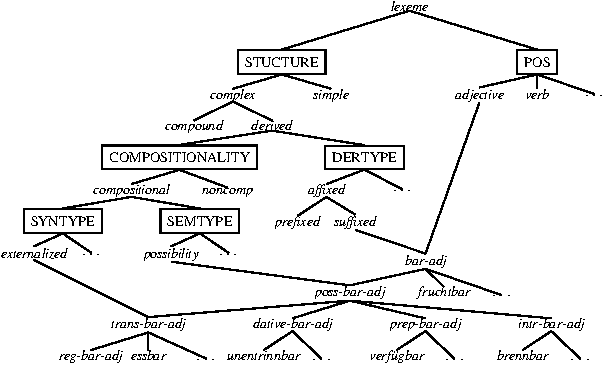
\includegraphics[scale=1.2]{figures/Riehemann-crop.pdf}
  
  \caption{Riehemann's type hierarchy of German \textit{-bar} derivation}
  \label{fig:Riehemann}
\end{figure}

She concludes that multiple inheritance type hierarchies lend
themselves towards capturing the variety of the full empirical pattern
while at the same time providing the necessary abstraction in terms of
more general supertypes from which individual subclasses may inherit. 



\newbox\poss
\newbox\suffixed
\newbox\externalised

\setbox\poss=\hbox{
  \avmoptions{active}
  \begin{avm}
    [\asort{possibility}
    ss|l|cont|nuc|reln & $\diamond$]
  \end{avm}
}
\setbox\suffixed=\hbox{
  \avmoptions{active}
  \begin{avm}
    [\asort{suffixed}
    ph & @1 $\oplus$ \normalfont\textit{list}\\
    morph-b & <[ph & @1]>]
  \end{avm}
}
\setbox\externalised=\hbox{
  \avmoptions{active}
  \begin{avm}
    [\asort{externalised}
    ss & [l|cat|val|subj &  <NP:@1>]\\
    morph-b  & <[ss|l|cat|val|comps & <NP\[\textit{acc}\]:@1,...>]>]
  \end{avm}
}

\begin{exe}
  \ex     \avmoptions{active}
  \begin{avm}
    [\asort{reg-bar-adj}\\
    ph & @1 + \textit{bar}\\
    morph-b & <[\asort{trans-verb}
    ph & @1\\
      ss|l & [cat|val|comps  <NP\[acc\]$_{@2}$> ~$\oplus$ @3]\\
      cont|nuc & @4[act & \textit{nom-obj}\\
      und & @2]]>\\
    ss|loc & [cat & [head & \textit{adj}\\
    val & [subj & <\normalfont NP$_{@2}$>\\
    comps & @3]]\\
    cont|nuc & [reln & $\diamond$\\
    und & @2\\
    soa-arg & @4]]]
  \end{avm} \label{fig:riehemannBar}
\end{exe}

Figure~\ref{fig:Riehemann} provides the extended hierarchy suggested
by \citet{Riehemann98}. The type for regular \textit{-bar} adjectives
given in (\ref{fig:riehemannBar}) is treated as a specific subtype
that inherits inter alia from more general supertypes that capture the
salient properties that characterise the regular formation, but which
also hold to some extent for subregular \textit{-bar} adjectives. 

  
One property that is almost trivial concerns suffixation of
\textit{-bar}, and it holds for the entire class.  

\begin{exe}
  \ex \usebox{\suffixed} \label{fig:riehemannSuff}
\end{exe}


\begin{sloppypar}
  A property which is common to most \textit{-bar} adjectives in
  German is that they denote ``possibility''. 
\end{sloppypar}

\begin{exe}
  \ex \usebox{\poss}
\end{exe}

Clearly more specific is the passivisation effect observed with
transitive bases.  

\begin{exe}
  \ex \usebox{\externalised}
\end{exe}

Regular \textit{-bar} adjectives (\ref{fig:riehemannBar}) inherit from all these supertypes, which
accounts for most of their properties, while at the same time
capturing the relatedness to sub-regular formations. 


One aspect that Riehemann's approach does not capture as part of the
grammar is the productivity of the regular
pattern. \citet{Riehemann98} suggests that this could be accounted for
by extra-grammatical properties, such as lexical frequency. Cf. also
Chapter~\crossrefchaptert{cxg} for further discussion.

\subsection{\citet{Koenig99}}

Koenig's work on lexical relations has made several important
contributions to our understanding of morphological processes within
the HPSG lexicon. Based on joint work with Dan Jurafsky
\citep{Koenig94}, he uses Online Type Construction (OTC) to turn the
hierarchical lexicon, which is actually a static system into a
dynamic, generative device. This enables him in particular to make a
systematic distinction between open types for regular, productive
formations, and closed types for subregular and irregular ones.

\citet{Koenig99} takes issue with the early conception of lexical
rules as meta-level rules either deriving an expanded lexicon from a
base lexicon (generative lexical rules), or else establishing
relations between items within the lexicon (redundancy rules). He
argues on the basis of grammatical function change, such as the
English passive, that systematic alternations are amenable to
underspecification in the hierarchical lexical,  once
cross-classification between types can be performed dynamically.

Online Type Construction depends on a hierarchical lexicon that is
organised into an  AND/OR network of conjunctive dimensions and
disjunctive types. While in a standard type hierarchy any two types
that do not have a common subtype are understood as incompatible, OTC
derives new subtypes by intersection of leaf types from different
dimensions. Leaf types within the same dimension are still considered
disjoint. Thus, dimensions define the range of inferrable
cross-classifications between types, without having to statically list
these types in the first place.

In Koenig's conception of the lexicon as a type underspecified
hierarchical lexicon (TUHL), the unexpanded lexicon is just a system of
types. Concrete lexical items, i.e. instances, are inferred from these
by means of OTC. 

Let us briefly consider a simple example for the active/passive
alternation: the minimal lexical type hierarchy is organised into two
dimensions, one representing specific lexemes, the other specifying
active voice and passive voice linking patterns for lexemes. Concrete
lexical items are now derived by cross-classifying exactly one leaf
type from one dimension with exactly one leaf type from the other.

\begin{figure}[htb]
  \centering
  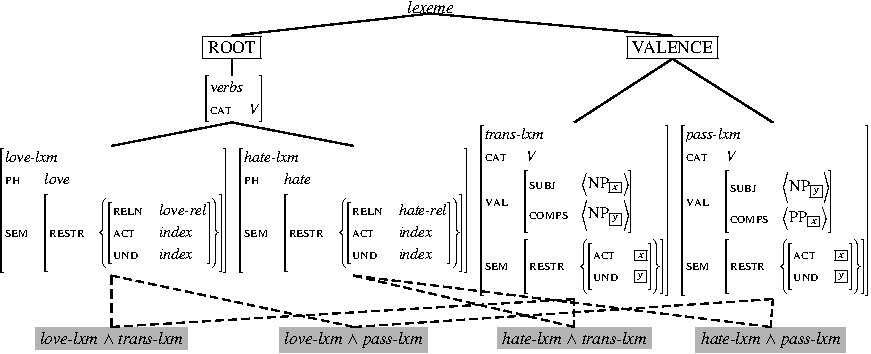
\includegraphics[scale=.84]{figures/OTC-crop.pdf}
  
  \caption{Online type construction}
  \label{fig:KoenigDyn}
\end{figure}
% Ex. love/hate -> kill/resurrect 

An important aspect of this integration of alternations
into the hierarchical lexicon is that it becomes quite straightforward 
to deal with lexical exceptions in a systematic way. The key to this
is pre-typing: e.g. in English, some transitive verbs, like possessive
\textit{have} fail to undergo passivisation. Rather than marking these
diacritically by features, pre-typing to the active pattern precludes
cross-classification with the passive pattern, since leaf types with a
dimension are disjoint and pre-typing makes this type already a leaf
type in both dimensions. 

\begin{figure}[htb]
  \centering
  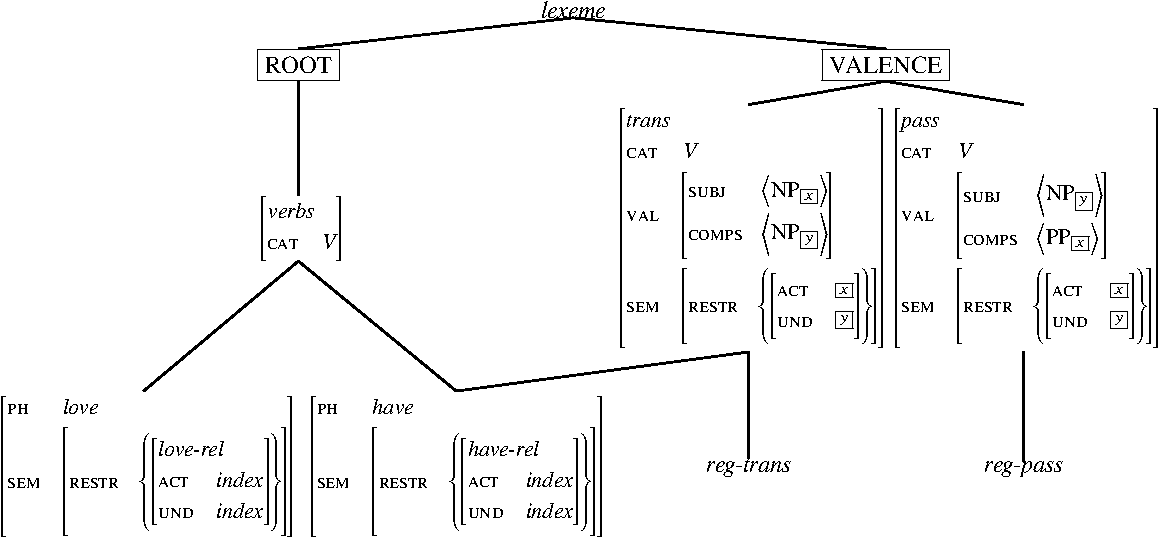
\includegraphics[scale=.63]{figures/pretyping-crop.pdf}

  \caption{Exceptions via pre-typing}
  \label{fig:KoenigPre}
\end{figure}

% Ex. pretyping



Online Type Construction successfully integrates systematic
alternations into type hierarchies. A crucial limitation is, however,
that OTC is confined to finite domains: by itself, it is suitable for
inflection and quasi-inflectional, non-recursive processes as
grammatical function change, while a full treatment of derivational
processes will still require recursive rule types, which remains a
possibility in Koenig's general approach to derivational morphology. 

\bigskip\noindent
The works of \citet{Riehemann98} and \cite{Koenig99} had considerable
impact on subsequent work on word formation, both within the framework 
of HPSG and beyond. Within HPSG, several studies of French derivation
and compounding directly build on these proposals \citep[e.g.][]{Tribout10,Desmets09}. 
Outside, the development of Construction Morphology
\citep{Booij10} has largely been influenced by the HPSG work on word
formation within a hierarchical lexicon. 

\section{Inflection}
\label{sec:Infl}

\subsection{Classical challenges of inflectional systems}
\label{sec:InflChallenges}

Ever since \citet{Matthews72}, it has been recognised in morphological
theory that inflectional systems do not privilege one-to one relations
between function and form, but must rather be conceived of as
many-to-many ($m:n$) in the general case. Thus, while
rule-by-rule compositionality can count as the success story
of syntax and semantics, this does not hold in the same way for inflection. 

Classical problems that illustrate the many-to-many nature of
inflection include cumulation, where a single form expresses multiple
morpho-syntactic properties. An extreme example of cumulation is
contributed by the Latin verb \textit{am-o}
`love-1.\textsc{sg}.\textsc{prs}.\textsc{ind}.\textsc{av}'. 

The mirror image of cumulation is extended (or multiple) exponence:
here, a single property is expressed by more than one exponent. This
is exemplified by German circumfixal past participles, such as
\textit{ge-setz-t} `\textsc{ppp}-sit-\textsc{ppp}', which is
 marked by a prefix \textit{ge-} and a suffix \textit{-t},
jointly expressing the perfect/passive participial property. Another
case of multiple exponence is contributed by Nyanja, whic marks
certain adjectives with a combination of two agreement markers, as
discussed on page \pageref{Nyanja} in
Section~\ref{sec:Panini}.  See
\citet{caballero_g-harris_a12} and \citet{Harris17} for a typological overview. 

Possibly more widely attested than pure multiple exponence is
overlapping exponence: e.g. many German nouns form the dative plural
by suffixation of \textit{-n}, but plural marking is often signalled
additionally by stem modification (\textit{Umlaut}): while \textit{Mutter-n}
`nut-\textsc{dat.pl}' merely shows cumulation of case and number,
\textit{Mütter-n} `mother.\textsc{pl}-\textsc{dat.pl}' exhibits plural
marking in both the inflectional ending and the fronting of the stem
vowel (cf. singular \textit{Mutter} `mother.\textsc{sg}').     

An extremely wide-spread form of deviation from a one-to-one
correspondence between form and function is zero exponence, where some
morpho"=syntactic properties do not give rise to any exponence. In
German, nouns inflect for four cases and two numbers, yielding
eight cells. However, in some paradigms only very few cells are
actually overtly marked. The feminine noun \textit{Mutter} `nut' does
not take any inflectional markings except in the dative plural
(\textit{Mutter-n} `nut-\textsc{dat.pl}'). Similarly, one of the most
productive masculine/neuter paradigms, witnessed by \textit{Rechner}
`computer', only shows overt marking for two cells, the genitive
singular (\textit{Rechner-s}) and the dative plural
(\textit{Rechner-n}), all other forms being bare.



The many-to-many nature of inflectional morphology clearly has
repercussions on how the system is organised.  One way to make sense
of inflection is in terms of paradigmatic opposition: i.e. while it
may be hard to figure out what exactly the meaning is of zero
case/number marking in German, we can easily establish the meaning of
a form like \textit{Rechner} in opposition to the non-bare forms
\textit{Rechner-s} `computer-\textsc{gen.sg}' and \textit{Rechner-n}
`computer-\textsc{dat.pl}'. This is even more the case, once we
consider different paradigms, i.e. different patterns of
opposition: e.g. the bare form \textit{Mutter} `nut' has a wider
denotation than \textit{Rechner} just because the latter stands in opposition
to fewer forms. 

The recognition of paradigms has led to number of works on syncretism
\citep[see, e.g.][]{Baerman05}, i.e. cases of systematic or accidental
identity of form across different cells of the paradigm. Syncretism
can give rise to splits of different types \citep{Corbett15}: natural splits, where
syncretic forms share some (non-disjunctive) set of features, Pāṇinian
splits, where syncretism corresponds to some default form, and finally
morphomic splits, where syncretic forms neither form a natural class
nor do they lend themselves to be analysed as a default. 

\begin{table}[htb]
  \centering
  
  \begin{subfigure}{.45\textwidth}
    \begin{tabular}{r|ll}
      \toprule
      & \textsc{singular} & \textsc{plural}\\
      \midrule
      \textsc{nom} & Oma & Oma-s\\
      \textsc{gen} & Oma & Oma-s\\
      \textsc{dat} & Oma & Oma-s\\
      \textsc{acc} & Oma & Oma-s\\
      \bottomrule
    \end{tabular}

    \caption{Natural split}
  \end{subfigure}  
  \begin{subfigure}{.45\textwidth}
    \begin{tabular}{r|ll}
      \toprule
      & \textsc{singular} & \textsc{plural}\\
      \midrule
      \textsc{nom} & Rechner & Rechner\\
      \textsc{gen} & Rechner-s & Rechner\\
      \textsc{dat} & Rechner & Rechner-n\\
      \textsc{acc} & Rechner & Rechner\\
      \bottomrule
    \end{tabular}
    \caption{Pāṇinian split}
  \end{subfigure}

  \begin{subfigure}{.45\textwidth}
      \begin{tabular}{r|ll}
        \toprule
        & \textsc{singular} & \textsc{plural}\\
        \midrule
        \textsc{nom} & Auto & Auto-s\\
        \textsc{gen} & Auto-s & Auto-s\\
        \textsc{dat} & Auto & Auto-s\\
        \textsc{acc} & Auto & Auto-s\\
        \bottomrule
      \end{tabular}
      \caption{Natural \& Pāṇinian split}
    \end{subfigure}
  \begin{subfigure}{.45\textwidth}
    \begin{tabular}{r|ll}
      \toprule
      & \textsc{singular} & \textsc{plural}\\
      \midrule
      \textsc{nom} & mur-s & mur\\
      \textsc{acc} & mur & mur-s\\
      \bottomrule
    \end{tabular}

    \caption{Morphomic split (Old French)}
  \end{subfigure}
  
  
  \caption{Paradigmatic splits}
  \label{tab:ParaSplit}
\end{table}

In Table~\ref{tab:ParaSplit}a, we find a perfect alignment of
syncretic forms along the number dimension. By contrast,
Figure~\ref{tab:ParaSplit}b illustrates the case discussed above,
where two specific cells constitute overrides to a general default
pattern (here: zero exponence). Default forms need not involve zero
exponence. German features a Pāṇinian split in another paradigm where
all forms are marked with \textit{-en} (e.g. \textit{Mensch-en}
`human(s)'), except the nominative singular (\textit{Mensch}
`human\textsc{.nom.sg}'), which constitutes a zero
override. Table~\ref{tab:ParaSplit}c illustrates how a Pāṇinian split
in the singular can combine with a natural split between singular and
plural. Finally, Figure~\ref{tab:ParaSplit}d witnesses what could be
taken as a morphomic split, where there is no natural alignment
between form and function, and no clear way to establish what is the
default and what is the override.

The patterns we have just seen have two clear implications for
morphological theory: first,  morphologists generally believe that
a version of Pāṇini's Principle, whereby more specific forms can block
more general ones, must be part of morphological theory, since
otherwise many generalisations will be lost. 
Second, the many-to-many nature of exponence has a direct impact on
the representation of inflectional meaning, which we will explore in
the next two subsections. 

\subsection{Typology of inflectional theories}
\label{sec:InflTypology}

Current morphological theories differ as to how they establish the
relation between a complex form and its parts and how this relation
determines the relation between form and function. The classical
morpheme-based view of morphology, where inflectional meaning is a
property of lexical items, constitutes the text book case of what
\cite{Hockett54} has dubbed the Item-and-Arrangement (IA) model.  The
general criticism that has been raised against such models is that
they fail to recognise the paradigmatic structure of inflectional
morphology and furthermore need to make extensive appeal to zero
morphemes (see \citealp{Anderson92} for a systematic criticism).

The alternative model \citet{Hockett54} discusses is the
Item-and-Process (IP) model where inflectional meaning is introduced
syncategorematically by way of rule application. Such approaches
are less prone to have difficulties with non-concatenative processes
like modification and zero exponence. However, IP approaches still do
not recognise the $m:n$ nature of inflectional morphology and are
therefore expected to have problems with e.g. multiple exponence. 


As a reaction to \citet{Matthews72}, new approaches to inflectional
morphology were developed taking the notion of paradigms much more
seriously. Theories, such as A-Morphous Morphology \citep{Anderson92}
or Paradigm Function Morphology \citep{Stump01} have been classified
into the Extended Word-and-Paradigm (WP) category.     

% A much more fine-grained typology of approaches to inflection that
% does more justice to the kind of theories currently on the market has
% been proposed more recently by \citet{Stump01}. His classification is
% two-fold, distinguishing approaches as to (i) whether they associate
% inflectional meaning with the word (\textit{inferential}), or
% morphemes (\textit{lexical}), and (ii) whether composition is
% information-increasing (\textit{incremental}) or not
% (\textit{realisational}). Classical morpheme-based theories like
% \citet{Lieber92} or \citet{Wunderlich95} are lexical-incremental:
% being incremental, they have problems accounting for multiple
% exponence, a problem shared by the inferential-incremental model
% proposed  in \citet{Steele95}.    

% Lexical-realisational

\subsection{HPSG approaches to inflection}
\label{sec:InflHPSG}

Over the years, several different proposals have been made as to the
treatment of inflectional morphology in HPSG. From the point of view
of the logic, there is no a priori expectation as to the type of model
(IA, IP, WP) that would be most compatible with HPSG's basic
assumptions. Indeed, any of the three models have been proposed at
some point. However, the arguments against morpheme-based models put
forth by \citet{Matthews72}, \citet{Spencer91}, \citet{Anderson92} and
\citet{Stump01} have been taken quite seriously within the HPSG
community, such that there is a clear preference for IP or WP models over
IA, notable exceptions being \citet{van-eynde_f94} and, more
recently, \citet{Emerson15}.

One of the most common ways to express lexical alternations is by
means of (description-level) lexical rules. Morpho-phonological changes
effected by such a rule are typically effected by some (often
undefined) function on the phonology of the daughter. Since
morphological marking is tied directly to rule application, approaches
along these lines constitute an instance of an IP model of
morphology. Work on morphology in grammar implementation typically
follows this line: e.g. in platforms like the LKB \citep{Copestake02},
character unification serves to provide statements of
morpho-phonological changes that can be attached to (unary) lexical
rules. See \citet{Goodman10} for a proposal as to how requirements for
certain inflections and dependencies
between morphological rules, e.g. the parts of extended or overlapping
exponence can be captured in a more systematic way,
and \citet{Crysmann:15:JLM,Crysmann:2017:JOMO} for implementations of
non-concatenative morphology. 


A notable exception to the function approach is the work of Olivier
Bonami: in a series of papers, he argued for the incorporation of a
serious formal model of morphology, namely PFM \citep{Stump01}, and
showed specifically that the integration should be done at the level
of the word, rather than individual lexical rules, in order to reap
the benefits of a WP model over an IP model.  In a similar vain,
\citet{Erjavec94} explores how a model such as PFM can be cast in
typed feature descriptions and observes that the only non-trivial
aspect of such an enterprise relates to Pāṇinian competition, which
requires a change to the underlying logic. See Section
\ref{sec:Panini} for detailed discussion.

In the area of cliticisation, several sketches of WP models have been
proposed: e.g. \citet{Miller97} provide an explication of the function
that realises the pronominal affix cluster, but the proposal was never
meant to scale up to a full formal theory of
inflection. \citet{crysmann_b03book} suggested a realisational,
morph-based model of inflection. While certainly more worked out, the
approach was certainly optimised for the treatment of clitic
clusters. 



\subsubsection{Word-based approaches}

\paragraph*{\citet{Krieger:Nerbonne:93}}
As stated earlier, probably one of the first approaches to morphology
in HPSG has been developed by \citet{Krieger:Nerbonne:93}. What they
propose is essentially an instance of a WP model, since they use
distributed disjunctions to directly represent entire paradigms,
matching exponents with the features they express. Most interestingly,
their approach to inflection contrasts quite starkly with their
work on derivation \citep{Krieger:Nerbonne:93}, which is essentially a
word-syntactic, i.e. morpheme-based approach.


\begin{table}[htb]
  \centering
  \begin{tabular}{r|cc}
    \toprule
    & \textsc{sg} & \textsc{pl}\\
    \midrule
    1 & -e & -n\\
    2 & -st & -t\\
    3 & -t & -n\\
    \bottomrule
  \end{tabular}
  \caption{Regular present indicative endings for  German verbs}
  \label{tab:GermanEndings}
\end{table}

Figure \ref{fig:DistrDisj} represents an encoding of the present
indicative paradigm for German (cf. the endings in Table
\ref{tab:GermanEndings}. The distributed disjunction, marked by ${\$
  1}$, associates each element in the disjunctive \textsc{ending}
value with the corresponding element in the disjunctive \textsc{agr}
value.  


\begin{figure}[htb]
  \centering

  \begin{avm}
    \[morph & \[stem & \@2\\
        ending & \@3 \{ $_{\$1}$  \normalfont ``e'', ``st'', ``t'', ``n'', ``t'',
        ``n''\}\\
        form & \@2 $+$  \@3\]\\
      synsem & \[local|head|agr & \{$_{\$1}$ \[per & 1\\num & sg \], \[per & 2\\
        num & sg\], ... , \[per & 3\\num & pl\]\} \]\]
  \end{avm}
  
  \caption{Encoding paradigms by distributed disjunctions \citep{Krieger:Nerbonne:93}}
  \label{fig:DistrDisj}
\end{figure}

They further argue that partially regular formations, such as
\textit{sollen} `should', which has no ending in the first and third
singular can be captured by means of default inheritance, overriding
the \textsc{ending} value as in Figure~\ref{fig:DistrDisjSollen}.  

\begin{figure}[htb]
  \centering

  \begin{avm}
    \[morph & \[ending & \{ $_{\$1}$ \normalfont ``'', ``st'', ``'', ``n'', ``t'',
        ``n''\}\]\]
  \end{avm}
  
  
  \caption{Partial irregularity by overriding default endings \citep{Krieger:Nerbonne:93}}
  \label{fig:DistrDisjSollen}
\end{figure}

Suppletive forms, as for auxiliary \textit{sein} `be' will equally
inherit from Figure~\ref{fig:DistrDisj}, yet override the form value.  

\begin{figure}[htb]
  \centering

  \begin{avm}
    \[morph & \[form & \{ $_{\$1}$ \normalfont ``bin'', ``bist'', ``ist'', ``sind'', ``seid'',
        ``sind''\}\]\]
  \end{avm}
  
  \caption{Suppletive verbs \citep{Krieger:Nerbonne:93}}
  \label{fig:DistrDisj}
\end{figure}

The approach by \citet{Krieger:Nerbonne:93} has not been widely
adopted, partially because few versions of HPSG support default
inheritance and even fewer support distributed
disjunctions. \citet[176--178]{Koenig99} also argues against distributed
disjunctions on independent theoretical grounds, suggesting that the
approach will not scale up to morphologically more complex systems.  

\paragraph*{\citet{Koenig99}}

Similar to \citet{Krieger:Nerbonne:93}, \citet{Koenig99} pursues a
word-based approach to inflection, in contrast to the IP approach he
developed for derivation. He focuses on the distinction between
regular, sub-regular and irregular formations and explores how these
can be represented in a systematic way in lexical type hierarchies
using Online Type Construction.

He departs from the observation that words  inflect along a finite number
of different inflectional dimensions and that within each dimension,
pairings of exponents and morpho-syntactic features stand in
paradigmatic opposition. Furthermore, neither completely uninflected
roots, nor partially derived words (e.g. lacking agreement
information) shall be able to function as lexical signs, so it is
necessary to enforce that inflection be applied. The and/or
logic of dimensions and types he proposed appears to be very
well-suited to account for these properties. 

\begin{table}
\setlength{\tabcolsep}{.3em}
\centering
\begin{tabular}{llllll}
\toprule 
 & \textsc{pos} & \textsc{neg}     &             & \textsc{pos} & \textsc{neg}\\
\midrule 
\textsc{1sg} & ni-{ta}-tak-{a} & \textbf{{si}}-{ta}-tak-{a}        & \textsc{1pl} & tu-{ta}-tak-{a}     & {ha}-tu-{ta}-tak-{a}\\
\textsc{2sg} & u-{ta}-tak-{a} & {ha}-u-{ta}-tak-{a}        & \textsc{2pl} & m-{ta}-tak-{a}      & {ha}-m-{ta}-tak-{a}\\
\textsc{3sg.m/wa} & a-{ta}-tak-{a} & {ha}-a-{ta}-tak-{a}    & \textsc{3pl.m/wa} & wa-{ta}-tak-{a} & {ha}-wa-{ta}-tak-{a}\\ 
\textsc{3sg.ki/vi} & ki-{ta}-tak-{a} & {ha}-ki-{ta}-tak-{a} & \textsc{3pl.ki/vi} & vi-{ta}-tak-{a} & {ha}-vi-{ta}-tak-{a}\\
etc. & &\\
\bottomrule
\end{tabular}
\caption{Future forms of the Swahili verb  \textsc{taka} ‘want’}
\label{tab:SwahiliPast}
\end{table}


For illustration, let us consider a subset of his analysis of Swahili
verb inflection. As shown in Table~\ref{tab:SwahiliPast}, Swahili
verbs (minimally) inflect for polarity, tense and subject
agreement.\footnote{The full paradigm recognises inflection for object
agreement and relatives, but this shall not concern us here, it being
sufficient that inflectional paradigms may be large but finite.} 

Because of this property, \citet{Koenig99} suggests that the
inflectional morphology of Swahili can be directly described at the
word level. He proposes a type hierarchy of word level inflectional
constructions as given in Figure~\ref{fig:KoenigSwahili}. 

\begin{figure}[htb]
  \centering
\begin{forest}
[\emph{verb-infl}
	[2ND-SLOT,draw
    	[\emph{1sg},name=1sg
    		[\emph{1sg-pos}]
    	]
    	[\emph{3pl}]
   ]
	[1ST-SLOT,draw
		[\emph{neg}
			[\emph{1sg-neg},name=neg]
			[\emph{¬1sg-neg}]
		]
		[\emph{pos}]
	]
	[3RD-SLOT,draw
		[\emph{pst}
			[\emph{pos-pst}]
			[\emph{neg-pst}]
		]
		[\emph{fut}]
	]
]
\draw (1sg.south) to (neg.north);
\end{forest}
  \caption{Koenig's constructional approach to Swahili position classes}\label{fig:KoenigSwahili}
\end{figure}

As shown in Table~\ref{tab:SwahiliPast}, tensed verbs with plural
subjects take 3 prefixes in the negative and two in the positive, with
the exponent of negative preceding the exponent of subject agreement,
preceding in turn the exponent of tense. \citet{Koenig99} proposes
three dimensions of inflectional construction types that correspond to
the three positional prefix slots. Since dimensions are conjunctive, a
well-formed Swahili word must inherit from exactly one type in each
dimensions. As he states, the and/or logic of dimensions and types is
the declarative analogue of the conjunctive rule blocks and
disjunctive rules in A-morphous Morphology \citep{Anderson92}.

Types in the dimensions are partial word-level descriptions of
(combinations of) prefixes. As shown by the sample types in Figure
\ref{fig:KoenigNegPast}, these partial descriptions pair some
morpho-syntactic properties (\textsc{$\mu$-feat}) with constraints on
the prefixes: e.g. the type \textit{$\neg$1sg-neg} constrains the
first prefix slot to be \textit{ha}, while leaving the other slots
underspecified. These will be further constrained by appropriate types
from the other two dimensions. Likewise, the type \textit{1sg-pos},
constrains slot 2 to be \textit{ni}, but specifies the further
requirement that the verb be \textsc{[neg~$-$]}.    

\begin{figure}[htb]
  \centering
  
  \begin{subfigure}{.4\textwidth}
      \begin{avm}
        \[ph & \[aff & \[pref & \< \normalfont ha, ..., ... \>\]\]\\
          cat  & \[head & \[$\mu$-feat & \[neg & $+$ \]\]\]\]
      \end{avm}
      \caption{\textit{$\neg$1sg-neg}} 
    \end{subfigure}
  \begin{subfigure}{.52\textwidth}
      \begin{avm}
    \[ph & \[aff & \[pref & \< ..., \normalfont ni, ... \>\]\]\\
    cat  & \[head & \[$\mu$-feat & \[neg & $-$\\
    subj-agr & \[per & 1\\
    num & sg\]\]\]\]\]
\end{avm}
\caption{\textit{1sg-pos}}
\end{subfigure}

  \begin{subfigure}{.48\textwidth}

      \begin{avm}
    \[ph & \[aff & \[pref & \< \normalfont si, \< ~ \>, ... \>\]\]\\
    cat  & \[head & \[$\mu$-feat & \[neg & $+$\\
    subj-agr & \[per & 1\\
    num & sg\]\]\]\]\]
\end{avm}

    \caption{\textit{1-sg-neg}}
  \end{subfigure}

  \caption{Sample types for Swahili}
  \label{fig:KoenigNegPast}
\end{figure}

Pre-linking of types finally permits a straightforward treatment of
cumulation across positional slots: e.g. the type \textit{1sg-neg}
simultaneously satisfies requirements for the first and second slot,
constraining one of the prefixes to be portmanteau \textit{si}, the
other one to be empty. Thus, by adopting a constructional perspective
on inflectional morphology, \citet{Koenig99} can capture interactions
between different affix positions. There is, however, one important
limitation to a direct word-based perspective: situations where
exponents form the same set of markers may (repeatedly) co-occur
within a word cannot be captured without an intermediate level of
rules. Such a situation is found with subject and object agreement
markers in Swahili, so-called parallel position classes
\citep{Stump93,Crysmann:Bonami:2016}, as well as with exuberant
exponence in Batsbi \citep{Harris09,Crysmann:2018:Batsbi}. We shall
come back to the issue in Section~\ref{sec:ConstrGen}. Finally, since
exponents are directly represented on an affix list under Koenig's
approach, position and shape cannot always be underspecified
independently of each other, which makes it more difficult to
capture variable morphotactics (see Section~\ref{sec:Mortax}).


An aspect of (inflectional) morphology that \citet{Koenig99} pays
particular attention to is the relation between regular, sub-regular
and irregular formations. He approaches the issue on two levels: the
level of knowledge representation and the level of knowledge use. 

At the representational level, regular formations, e.g.\ past tense
\textit{snored}, are said to be intensionally defined in terms of
regular rule types that license them, i.e. results of regular rule
application are not listed in the lexicon. They are constructed either
by Online Type Construction or rule application.  Irregular
formations, by contrast are fully listed, e.g.\ the past tense form
\textit{took} of a verb like \textit{take}. Most interesting are
sub-regular types, e.g.\ \textit{sing/sang/sung} or
\textit{ring/rang/rung}: like irregulars, class membership is
extensionally defined by enumeration, but the type hierarchy can still
be exploited to abstract out common properties.

With regular formations being defined in terms of productive schemata,
an important task is to preempt any subregular or irregular root from
undergoing the regular, productive pattern. \citet{Koenig99} discusses
three different approaches in depth: a feature-based approach, and two
ways of invoking Pāṇini's Principle. As for the former, he shows that
the costs associated with diacritic exception features is actually
minimal, i.e. it is sufficient to specify irregular and subregular
bases as \textsc{[irr~$+$]} and constrain the regular rule to
\textsc{[irr~$-$]}. Thus, use of such diacritics does not need to be
stated for the large and open class of regular, productive
bases. Despite the relatively harmless effects of the feature-based
approach, it should be kept in mind that this approach will not scale
up to a full treatment of Pāṇinian competition.\footnote{This is
  because first, every default/override pair would need to be
  stipulated, and second, if a paradigm has defaults in different
  dimension (e.g. a default tense, or a default agreement marking),
  each would need its own diacritic feature.}

\citet{Koenig99} proposes two variants of a morphological and/or lexical blocking
theory. In essence, he builds on a previous formulation by
\citet{Andrews90} within LFG to define a notion of morphological
competition based on subsumption. Since competition is between
different realisations for the same morphological features, he applies
a restrictor on form-related features to then establish competition in
terms of uni-lateral subsumption ($\sqsubset$): i.e. a
rule-description that is more specific than some other rule (modulo
form-oriented features) will take precedence. I shall not go into the
details of Koenig's Blocking Principle here, since we shall come back
to a highly similar formulation of Pāṇinian competition in
Section~\ref{sec:Panini}.  \citet{Koenig99} discusses two different
ways how this can be accomplished: one is a compilation approach where
complementation is used to make the more general type disjoint, the
other relegates the problem to the area of knowledge use. While the
usage-based interpretation may appear preferable, because it does not
require expansion of the lexical type-hierarchy, it leaves open the
question why this kind of competition is mainly restricted to lexical
knowledge. On the other hand, the static compilation approach requires
prior expansion of the type underspecified lexicon in order to give
sound results under restriction, a point made in
\citet{crysmann_b03book}.

\bigskip\noindent To summarise, several WP proposals have been made to
replace the IP model tacitly assumed by many HPSG syntacticians, which
merely attaches some morpho-phonological function to a lexical rule.
Bonami \citep{Bonami08f,Bonami06,Bonami07e,Bonami11f} proposed to
directly plug-in a credible external framework, namely Paradigm
Function Morphology \citep{Stump01}, \citet{Koenig99} suggested a
word-based model. Neither approach has proven to be fully
satisfactory. Use of an external theory, such as PFM, not only begs
the question why we need a different formalism in order to implement a
theory of inflection, rather than exploit the power of inheritance and
cross-classification in hierarchies of typed feature structure
descriptions. Word-based approaches suffer from problems of
scalability with morphotactically complex systems.  These issues led
to the development of Information-based Morphology
\citep{Crysmann:Bonami:2016}, which will be discussed in the next
section.


\section{Information-based Morphology}
\label{sec:IbM}

Information-based morphology \citep{Crysmann:Bonami:2016} is a theory
of inflectional morphology that systematically builds on HPSG-style
typed feature logic in order to implement an inferential-realisational
model of inflection. As the name suggests in reference to
\citet{Pollard87}, it aims at complementing HPSG with a 
sub-theory of inflection that systematically 
explores underspecification and cross-classification as the central
device for morphological generalisations.

IbM clearly builds on previous HPSG work on morphology and the
lexicon: Online Type Construction \citep{Koenig94} can be cited here
in the context of the underlying logic. Similarly, the decision to
represent morphotactics in terms of a flat lists of segmentable
exponents (=morphs) draws on previous work by
\citet{crysmann_b03book}. 

% Brief comparison between IbM and PFM/AM

\subsection{Architecture and principles}

The architecture of IbM is quite simple: essentially, words are
assumed to introduce a feature \textsc{infl} that encapsulates all
features relevant to inflection. At the top-level, these comprise
\textsc{mph}, a partially ordered list of exponents (\textit{morph}),
a morphosyntactic (or morpho-semantic) property set \textsc{ms}
associated with the word, and finally a set of \textsc{rr} of
realisation rules that establish the correspondence between exponents
and morphosyntactic properties.   

\begin{exe}
  \ex
  \begin{avm}
    \[\asort{word}
      infl &
      \[mph & list({morph})\\
      rr & set(realisation-rule)\\
    ms & set(msp)\]\]
  \end{avm}

\end{exe}

From the viewpoint of inflectional morphology, words can be regarded
as associations between a phonological shape (\textsc{ph}) and a
morphosyntactic property set (\textsc{ms}), the latter including, of
course, information pertaining to lexeme identity. This correspondence
can be described in a maximally holistic fashion, as shown in 
(\ref{fig:Word}). Throughout this section, I shall use German
(circumfixal) passive/past participle (\emph{ppp}) formation, as
witnessed by \textit{ge-setz-t} `put', for illustration.

\begin{exe}
  \ex \begin{avm}
    \[ ph & \< \normalfont gesetzt\>\\
      infl & \[ms & \{\[lid & setzen\],\[tma & ppp\]\}\]
    \]
  \end{avm}
  
  \label{fig:Word}
\end{exe}

Since words in inflectional languages typically consist of multiple
segment\-able parts, realisational models provide means to index
position within a word: while in AM and PFM ordered rule blocks
perform this function, IbM uses a list of morphs (\textsc{mph}) in
order to explicitly represent exponence. 
%
% Having morphosyntactic
% properties and exponents represented as sets and lists, standard
% issues in inflectional morphology are straightforwardly captured at
% the level of rules: cumulative exponence corresponds to the expression
% of $m$ properties by 1 morph, whereas extended (or multiple) exponence
% corresponds to 1 property being expressed by $n$ morphs. Overlapping
% exponence finally represents the general case of $m$ properties being
% realised by $n$ exponents.
% Figure \ref{fig:WordMph} illustrates the
% word-level $m:n$ correspondence of lexemic and inflectional properties
% to the multiple morphs that realise it. 
The sample word-level representation in (\ref{fig:WordMph})
illustrates the kind of information represented on the \textsc{mph}
list and the \textsc{ms} set. While elements of the \textsc{ms} set
are either inflectional features or lexemic properties, the latter comprising
e.g. information about the stem shape or inflection class membership,
\textsc{mph} is a list of structured elements consisting of a
phonological description (\textsc{ph}) paired with a position class
index (\textsc{pc}).   

\begin{exe}
  \ex \textit{mph} $\rightarrow$
  \begin{avm}
    \[ph & list(phon)\\
      pc & pos-class\]
  \end{avm}

\end{exe}

The reification of position and shape as first class citizens of
morphological representation is one of the central design decisions of
IbM: as a result, constraints on position and shape will be amenable
to the very same underspecification techniques as all other
morphological properties. As a consequence, IbM eliminates structure
from inflectional morphology, which clearly distinguishes this
approach from other inferential-realisational approaches, such as PFM
or AM, where order is derived from cascaded rule application.

\begin{exe}
  \ex Structured association of form (\textsc{mph}) and function (\textsc{ms})   \label{fig:WordMph}

  \begin{xlist}
    \ex Word:

    \begin{avm}
      \[mph & \<\[ph &  <ge>\\ pc & -1\],\[ph &  <setz>\\ pc & 0\],\[ph &  <t>\\ pc & 1\]\>\\
        ms & \{\[lid & setzen\],\[tma & ppp\]\}
      \]
    \end{avm}
    \ex Abstraction of circumfixation ($1:n$):

    \begin{avm}
      \[ mph & \<\[ph &  <ge>\\ pc & -1\],\[ph &  <t>\\ pc & 1\],\ldots\>\\
        ms & \{\[tma & ppp\],\ldots\}
      \]
    \end{avm}
  \end{xlist}
\end{exe}

By means of underspecification, i.e. partial descriptions, one can
easily abstract out realisation of the past participle property,
arriving at a direct word-based representation of circumfixal
realisation, as shown in (\ref{fig:WordMph}).  Yet, a direct
word-based description does not easily capture situations where the
same association between form and content is used more than once in
the same word, as is arguably the case for Swahili
\citep{Stump93,Crysmann:Bonami:2016,Crysmann:Bonami:2017:HPSG} or,
even more importantly for Batsbi \citep{Harris09}.

By way of introducing a level of \textsc{r(ealisation) r(ules)}, reuse
of resources becomes possible. Rather than expressing the relation
between form and function directly at the word level, IbM assumes that
a word's description includes a specification of which rules license
the realisation between form and content, as shown in 
(\ref{fig:WordRR}).


\begin{exe}
  \ex{Association of form and function mediated by rule}

  \begin{avm}
    \[ mph & \<\rnode{xx}{\[ph &  <ge>\\ pc & -1\]} \rnode{aa}{\[ph &  <setz>\\ pc & 0\]},\rnode{ab}{\[ph &  <t>\\ pc & 1\]}\> \\
      rr & \{	\[	mph & \{\rnode{ba}{\[ph &  <setz>\\ pc & 0\]}\}\\
        mud & \{\rnode{ca}{\[lid & setzen\]}\}
      \],
      \[	mph & \{\rnode{yy}{\[ph &  <ge>\\ pc & -1\]},\rnode{bb}{\[ph &  <t>\\ pc & 1\]}\}\\
        mud & \{\rnode{cb}{\[tma & ppp\]}\}
      \]
      \}	\\ \\
      ms & \{\rnode{da}{\[lid & setzen\]},\rnode{db}{\[tma & ppp\]}\}
    \]
  \end{avm}
  \psset{arrows=<->,linecolor=gray,linestyle=dotted,angleA=-90,angleB=90}
  \nccurve{xx}{yy} \nccurve{aa}{ba} \nccurve{ab}{bb} \nccurve{ca}{da}
  \nccurve{cb}{db}

\label{fig:WordRR}
\end{exe}

Recognition of a level of realisation rules that mediate between parts
of form and parts of function slightly increases the complexity of
morphological descriptions beyond a simple pairing of form-related
\textsc{mph} lists and function-related \textsc{ms} sets. 

The crucial point about realisation rules is that they take care of
parts of the inflection of an entire word independently of other
realisation rules. Thus, in IbM, realisation rules explicitly
represent the subset of morphosyntactic  features they are
about. I.e. realisation rules introduce a feature \textsc{mud}
(=Morphology Under Discussion), in addition to \textsc{mph} and
\textsc{ms}, in order to single out the morphosyntactic features that
are licensed by application of the rule.

\begin{exe}
  \ex
  \textit{realisation-rule} $\rightarrow$ \begin{avm}
    \[mud & \@1 set(msp)\\
      ms & \@1 ~$\cup$ set(msp)\\
    mph & list(morph)\]
  \end{avm}

\end{exe}

Realisation rules (members of set \textsc{rr}) pair a set of
morphological properties to be expressed, the morphology under
discussion (\textsc{mud}), with a list of morphs that realise them
(\textsc{mph}). Since \textsc{mud}, being a set, admits multiple
morphosyntactic properties, and since \textsc{mph}, being a list
admits multiple exponents, realisation rules are fully $m:n$. This
property sets this framework apart from cascaded rule models of
inferential-realisational morphology \citep{Anderson92,Stump01}, which
attain this property indirectly based on cascaded rules that are
basically $m:1$.

\begin{figure}[htb]
  \begin{center}

    \textit{word} $\rightarrow$
    \begin{avm}
       \[mph & \@{e$_1$} $\bigcirc\dots\bigcirc$ \@{e$_n$}\\
         rr & \{ \[mph & \@{e$_1$}\\mud & \@{m$_1$}\\ms & \@0\] ,\ldots\ ,
         \[mph & \@{e$_n$}\\mud & \@{m$_n$}\\ ms & \@0\] \}\\
         ms & \@{m$_1$} $\uplus\dots\uplus$ \@{m$_n$}
        \]
    \end{avm}
      \end{center}
  \caption{Morphological well-formedness}
  \label{fig:MCC}
\end{figure}

Given two distinct levels of representation, the morphological word
and the rules that license it, it is of course necessary
to define how constraints contributed by realisation rules relate to
the overall morphological makeup of the word. Realisation rules per se
only provide recipes for matching morphosyntactic properties onto
exponents and vice versa. In order to describe well-formed words, it
is necessary to enforce that these recipes actually be applied. IbM
regulates the relation between word-level properties and realisation
rules by means of  rather straightforward principle, given in
Figure~\ref{fig:MCC}: this very general principle of morphological well-formedness  ensures that the properties expressed by rules add up
to the word's property set and that the rules' \textsc{mph} lists add
up to that of the word, i.e. no contribution of a rule may ever be
lost. This principle of general well-formedness in
Figure~\ref{fig:MCC} bears some resemblance to LFG's principles of
completeness and coherence \citep{bresnan_j82}, as well as to the
notion of `Total Accountability' proposed by \citet{Hockett47}. Since
$m:n$ relations are recognised at the most basic level,
i.e. morphological rules, mappings between the contributions of the
rules and the properties of the word can and should be $1:1$.

In essence, a word's morphosyntactic property set (\textsc{ms}) will
correspond to the non-trivial set union ($\uplus$) of the rules'
\textsc{mud} values.\footnote{While standard set union ($\cup$) allows
  for the situation that elements contributed by two sets may be
  collapsed, non-trivial set union ($\uplus$) insists that the sets to
  be unioned must be disjoint.}  The entire morphosyntactic
property set of the word (\textsc{ms}) is exposed on each realisation
rule by way of structure sharing (\avmbox{0}). 

Finally, a word's sequence of morphs, and hence: its phonology, will
be obtained by shuffling ($\bigcirc$) the rules' \textsc{mph} lists in
ascending order of position class (\textsc{pc}) indices. This is
ensured by the Morph Ordering Principle given in Figure~\ref{fig:MOP},
adapted from \citet{Crysmann:Bonami:2016}.


\begin{figure}[htb]
  \centering

  
  
  \begin{subfigure}{\textwidth}
    \centering
    \textit{word} $\rightarrow$\\
      \begin{avm}
        \[ph & \@1 $\oplus \dots \oplus$ \@n\\
          infl & \[mph & \<\[ph & \@1 \], $\dots$ \[ph & \@n \]
            \> \]\]
      \end{avm}
    \caption{Concatenation}
  \end{subfigure}
  
  \begin{subfigure}{\textwidth}
    \centering
      \textit{word}
    $\rightarrow$\\
    \begin{avm}
      $\neg$ \( \[infl & \[
          mph & \< ... \[pc & \@m  \], \[
            pc & \@n \],...\>
        \]\] ~$\wedge$ ~ \@m $\geq$ \@n\)
    \end{avm}
      \caption{Order}
    \end{subfigure}

    \caption{Morph Ordering Principle (MOP)}
  \label{fig:MOP}
\end{figure}

While the first clause in Figure~\ref{fig:MOP} merely states that the
word's phonology is the concatenation of its constituent morphs, the
second clause ensures that the order implied by position class indices
(\textsc{pc}) is actually obeyed. \citet{bonami_o-crysmann_b13hpsg}
provide a formalisation of morph ordering using list constraints.

Given the very general nature of the well-formedness constraints and
particularly the commitment to monotonicity embodied by
Figure~\ref{fig:MCC}, it is clear that most if not all of the actual
morphological analysis will take place at the level of realisation
rules.


\subsection{Realisation rules}

The fact that IbM, in contrast to PFM or AM, recognises $m:n$
relations between form and function at the most basic level of
organisation, i.e. realisation rules, means that morphological
generalisations can be expressed in a single place, name\-ly simply as
abstractions over rules. Rules in IbM are represented as descriptions
of typed feature structures organised in an inheritance hierarchy,
such that properties common to leaf types can be abstracted out into
more general supertypes. This vertical abstraction is illustrated in
Figure \ref{fig:Vertical}. Using again German past participles as an
example, the commonalities that regular circumfixal \textit{ge-...-t}
(as in \textit{gesetzt} `put') shares with subregular
\textit{ge-...-en} (as in \textit{geschrieben} `written') can be
generalised as the properties of a rule supertype from which the more
specific leaves inherit. Note that essentially all information except
choice of suffixal shape is associated with the supertype. This
includes the shared morphotactics of the suffix.

\begin{figure}
	\centering
%    \hspace*{-1em} 
\begin{forest}
%\psset{levelsep=8em,treesep=12em,linewidth=0pt,nodesep=0pt}
[{\begin{avm}
    \[mud & \{ \[tma & ppp\] \}\\
      mph & \< \[ph & ge\\ pc & -1 \],
      \[pc & 1 \] \> \]
  \end{avm}}
	[{\begin{avm}
		\[mph & \< ..., \[ph & t \] \> \]
	\end{avm}}]
	[{\begin{avm}
		\[mph & \< ..., \[ph & en 
		\] \>\]
	\end{avm}}]
]
\end{forest}
	\caption{Vertical abstraction by inheritance}\label{fig:Vertical}
\end{figure}

In addition to vertical abstraction by means of standard monotonic
inheritance hierarchies, IbM draws on Online Type Construction
\citep{Koenig94}: using dynamic cross-classification, leaf types from
one dimension are distributed over the leaf types of another
dimension. This type of horizontal abstractions permits modelling of
systematic alternations, as illustrated once more with German past
participle formation:

\begin{exe}
  \ex \label{ex:ppp}
  \begin{xlist}

    \ex \textbf{ge}-setz-\textbf{t} `set/put'
    \ex über-setz-\textbf{t} `translated'
    \ex \textbf{ge}-schrieb-\textbf{en} `written'
    \ex über-schrieb-\textbf{en} `overwritten'
  \end{xlist}
\end{exe}

In the more complete set of past participle formations shown in
(\ref{ex:ppp}), we find alternation not only between choice of suffix
shape (\textit{-t} vs. \textit{-en}), but also between presence
vs. absence of the prefixal part (\textit{ge-}).

\begin{figure}
  \centering
  \footnotesize
\begin{forest}
[{\begin{avm}
  \[mud & \{\[tma & ppp\]\}\\
    mph & \< ..., \[pc & 1\] \>\]
\end{avm}}
	[PREF,draw
		[{\begin{avm}
			\[mph & \< \[ph & ge\\pc & -1\], \[ ~ \]\>\]
		\end{avm}}]
		[{\begin{avm}
			\[mph & \< \[ ~ \] \> \]
		\end{avm}}]
	]
	[SUFF,draw
		[{\begin{avm}
            \[mph & \<..., \[ph & t\]\>\]
          \end{avm}}]
		[{\begin{avm}
			\[mph & \< ..., \[ph & en\]\>\]
		\end{avm}}]
	]
]
\end{forest}
  \caption{Horizontal abstraction by dynamic cross-classification}\label{fig:Horizontal}
\end{figure}

Figure \ref{fig:Horizontal} shows how Online Type Construction provides
a means to generalise these patterns in a straightforward way: while the
common supertype still captures properties true of all four different
realisations, namely the property to be expressed and the fact that it
involves at least a suffix, concrete prefixal and suffixal realisation
patterns are segregated into dimensions of their own (indicated by
\avmbox{PREF} and \avmbox{SUFF}). Systematic cross-classification
(under unification) of types in \avmbox{PREF} with those in
\avmbox{SUFF} yields the set of well-formed rule instances,
e.g. distributing the left-hand rule type in \avmbox{PREF} over the
types in \avmbox{SUFF} yields the rules for \textit{ge-setz-t} and
\textit{ge-schrieb-en}, whereas distributing the right hand rule type
in \avmbox{PREF} gives us the rules for \textit{über-setz-t} and
\textit{über-schrieb-en}, which are characterised by the absence of
the participial prefix.

Having illustrated how the kind of dynamic cross-classification
offered by Online Type Construction is highly useful for the analysis
of systematic alternation in morphology, it seems necessary to lay out
in a more precise fashion its exact workings. In its original
formulation by \citet{Koenig94,Koenig99}, OTC was conceived as a
closure operation on underspecified lexical type hierarchies. IbM
merely redeploys their approach for the purposes of inflectional
morphology. Essentially, a minimal type hierarchy as in
Figure~\ref{fig:Horizontal} provides instructions on the set of
inferrable sub-types: according to \citet{Koenig94}, dimensions are
conjunctive and leaf types are disjunctive. Online Type Construction
dictates that any maximal sub-type must inherit from exactly one leaf
type in each dimension. The maximal types of the hierarchy thus
expanded serve as the basis for rule instances, i.e. actual
rules.\footnote{\label{fn:OTC}There are two ways of conceptualising the status of
  OTC in grammar: under the dynamic view, hierarchies are
  underspecified and the full range of admissible type and therefore
  the range of instances is inferred online. Under the more
  conservative static view, the underspecified description is merely a
  convenient shortcut for the grammar writer. In either case,
  generalisations are preserved.   
   }



\subsection{Pāṇinian competition}
\label{sec:Panini}

In accord with most theories of inflection
\citep{Prince93,Stump01,Anderson92,Noyer92,kiparsky_p85}, IbM embraces
a version of Morphological Blocking, aka the Elsewhere Condition
\citep{kiparsky_p85} or Pāṇini's Principle. The basic intuition behind
Pāṇinian competition is that more specific rules can block the
application of more general rules, where the most unspecific rule will
count as a default. In terms of feature logic, the notion of
specificity corresponds to some version of the subsumption relation.

Competition between rules or lexical entries does not follow from the
logic standardly assumed within HPSG: if a rule can apply, it will
apply, no matter whether there are any more specific or more general
rules that could have applied as well (in fact, they would apply as
well). Thus, implementation of a notion of morphological blocking
necessitates a change to the logic.

As has been discussed already in \citet{Koenig99}, preemption based on
specificity of information can be either addressed statically (at
``compile-time'') as an issue of knowledge representation or
dynamically (at ``run-time'') as a question of knowledge
use. Independently of the choice between a static or dynamic version
of preemption, the main task is to provide a notion of competitor.  In
the interest of representing Pāṇinian inferences transparently in the
type hierarchy, IbM makes use of a closure operation on rule
instances, as detailed in (\ref{ex:PAN}), which is clearly inspired by
\citet{Koenig99} and \citet{Erjavec94}.\footnote{Alternatively, for 
a dynamic approach, it will be sufficient to use clause
(\ref{ex:PAN}a) and perform a topological sort on rule instances,
ordering  more specific rules before more general ones.}

\begin{samepage}
  \begin{exe}
    \ex \label{ex:PAN}\begin{description}
    \item[Pāṇinian Competition (PAN)] \mbox{~}
      \begin{xlist}
        \ex For any leaf type $t_1$[\textsc{mud} $\mu_1$,\textsc{ms}
        $\sigma$], $t_2$[\textsc{mud} $\mu_2$,\textsc{ms}
        $\sigma \wedge \tau$] is a morphological competitor, iff
        $\mu_1 \cup \mbox{\textit{set}} \sqsubseteq \mu_2 \cup \mbox{\textit{set}}$.
    
        \ex For any leaf type $t_1$ with competitor $t_2$, expand
        $t_1$'s \textsc{ms} $\sigma$ with the negation of $t_2$'s
        \textsc{ms} $\sigma \wedge \tau$:
        $\sigma \wedge \neg (\sigma \wedge \tau) \equiv \sigma \wedge
        \neg \tau$.
      \end{xlist}
    \end{description}
  \end{exe}
\end{samepage}

The first clause establishes competition, ensuring subsumption with
respect to both expressed features (\textsc{mud}) and conditioning
features (\textsc{ms} descriptions).\footnote{Since \textsc{mud} values
  can be of different cardinality, the subsumption  is checked
  on  open sets containing the original \textsc{mud} sets. } If the condition is met, the use
conditions of the more general rule are specialised in such a way as
to make the two rule descriptions fully disjoint.

% An example is needed here!

\begin{table}
\setlength{\tabcolsep}{.3em}
\centering
\begin{tabular}{llllll}
\toprule 
 & \textsc{pos} & \textsc{neg}     &             & \textsc{pos} & \textsc{neg}\\
\midrule 
\textsc{1sg} & ni-{ta}-tak-{a} & \textbf{{si}}-{ta}-tak-{a}        & \textsc{1pl} & tu-{ta}-tak-{a}     & {ha}-tu-{ta}-tak-{a}\\
\textsc{2sg} & u-{ta}-tak-{a} & {ha}-u-{ta}-tak-{a}        & \textsc{2pl} & m-{ta}-tak-{a}      & {ha}-m-{ta}-tak-{a}\\
\textsc{3sg.m/wa} & a-{ta}-tak-{a} & {ha}-a-{ta}-tak-{a}    & \textsc{3pl.m/wa} & wa-{ta}-tak-{a} & {ha}-wa-{ta}-tak-{a}\\ 
\textsc{3sg.ki/vi} & ki-{ta}-tak-{a} & {ha}-ki-{ta}-tak-{a} & \textsc{3pl.ki/vi} & vi-{ta}-tak-{a} & {ha}-vi-{ta}-tak-{a}\\
etc. & &\\
\bottomrule
\end{tabular}
\caption{Future forms of the Swahili verb  \textsc{taka} ‘want’}
\label{tab:SwahiliPortmanteau}
\end{table}

For concreteness, let us consider some examples from Swahili: as shown
in Table~\ref{tab:SwahiliPortmanteau}, the negative in Swahili is
typically formed by a prefix \textit{ha}, preceding the equally
prefixal exponents of
subject agreement and tense (future \textit{ta}). However, in the
negative first singular, discrete realisation of \textit{ha} and
\textit{ni} is blocked by the portmanteau \textit{si}. Here, we have
a classical case of   Pāṇinian competition, where a rule that
expresses both negative and first person singular agreement preempts
application of the more general individual rules for negative or first
person singular.  



In the case of \textit{si}, we find the portmanteau in the same
surface position as the exponents it is in competition with.  However,
this need not be the case, nor indeed is preemption of this kind
limited to adjacency. E.g.  relative negative \textit{si} is realised
in a position following the subject agreement marker, yet still, by
virtue of expressing negative in the context of relative marking, it
blocks realisation of negative \textit{ha} in pre-agreement position. This constitutes a case of what \citet{Noyer92} calls ``discontinuous
bleeding''. 

\begin{exe}
  \ex \label{ex:SwahiliNeg1sg}
  \begin{xlist}
    \ex[]{\gll {ha}- wa- ta- taka\\
      \textsc{neg} \textsc{sbj.pl.m/wa} \textsc{fut} want\\
      \glt `they will not want'}
    \ex[]{\gll watu wa- \textit{si-} o- soma\\
      people \textsc{sbj.pl.m/wa} \textsc{neg.rel} \textsc{rel.pl.m/wa} read\\
      \glt `people who don't read'}
    
    \ex[*]{\gll watu {ha-} wa- \textit{(si-)} o- soma\\
      people \textsc{neg} \textsc{sbj.pl.m/wa} \textsc{neg.rel} \textsc{rel.pl.m/wa} read\\
      \glt }
    
  \end{xlist}
\end{exe}

The relevant realisation rules for \textit{ha}, \textit{ni}, and the
two markers \textit{si}, can be formulated quite straightforwardly as
in (\ref{ex:SwahiliPanini}a--d), in that order. For expository
purposes, I shall make explicit the fact that \textsc{mud} is necessarily
contained in \textsc{ms}.   

\begin{exe}
  \ex \label{ex:SwahiliPanini}
  \begin{minipage}[t]{0.4\linewidth} \begin{xlist}
      \exi{a. \begin{avm}
          \[mud & \@1 \{ \normalfont\textit{neg}\/ \}\\
            ms & \@1 $\cup$ set\\
            mph & \< \[ph & \<\normalfont ha\>\\
              pc & $1$\] \> \]
        \end{avm}}
    \end{xlist}
  \end{minipage} ~ \begin{minipage}[t]{0.4\linewidth} \begin{xlist}
        \exi{b.  \begin{avm}
            \[mud & \@1 \{ \[\asort{ subj}
            per & 1\\num & sg\] \}\\
            ms & \@1 $\cup$ set\\
            mph & \< \[ph & \<\normalfont ni\>\\
            pc & 2\] \> \]
        \end{avm}}
    \end{xlist}
  \end{minipage}


\begin{minipage}[t]{0.4\linewidth} \begin{xlist}
      \exi{c.  \begin{avm}
          \[mud &  \@1 \{ \normalfont\textit{neg},\\ \[\asort{subj}
              per & 1\\num & sg\]\}\\
            mph & \< \[ph & \<\normalfont si\>\\
            pc & $3$\] \> \]
        \end{avm}}
    \end{xlist}
  \end{minipage}

\end{exe}

On the basis of the definition in (\ref{ex:PAN}a), portmanteau
\textit{si} in (\ref{ex:SwahiliPanini}c)\footnote{IbM uses the
  notation $m..n$ to represent spans of position classes. See
  \citet{bonami_o-crysmann_b13hpsg} for a proposal of how spans can be made explicit.} is a competitor for both
\textit{ni} (\ref{ex:SwahiliPanini}b) and \textit{ha}
(\ref{ex:SwahiliPanini}c), since the \textsc{mud} of portmanteau
\textit{si} is subsumed by either the set containing the \textsc{mud}
value of \textit{ni} or \textit{ha}. Moreover, the \textsc{ms} value
of portmanteau \textit{si} is properly subsumed by \textit{ni} (and
\textit{ha}). Accordingly, the rule for \textit{ni} will be expanded
as in (\ref{ex:PanExp}a).  Similarly, in a first iteration,
\textit{ha} will be specialised as in (\ref{ex:PanExp}b). 

\begin{exe}
  \ex \label{ex:PanExp}
  \begin{minipage}[t]{0.49\linewidth}
    \begin{xlist}
      \exi{a.
        \begin{avm}
          \[mud & \@1 \{ \[\asort{ subj}
              per & 1\\num & sg\] \}\\
            ms & \@1 $\cup$ set $\wedge$ $\neg$ \{ \normalfont\textit{neg}, ... \}\\
            mph & \< \[ph & \<\normalfont ni\>\\
              pc & 2\] \> \]
        \end{avm}}
    \end{xlist}
  \end{minipage}
  \begin{minipage}[t]{0.49\linewidth}
    \begin{xlist}
      \exi{b. \begin{avm}
          \[mud & \@1 \{ \normalfont\textit{neg} \}\\
            ms & \@1 $\cup$  $\neg$ \{ \[\asort{subj}
              per & 1\\num & sg\], ... \}\\
            mph & \< \[ph & \<\normalfont ha\>\\
              pc & 1\] \> \]
        \end{avm}
      }
    \end{xlist}
  \end{minipage}
\end{exe}

However, \textit{ha} (\ref{ex:SwahiliPanini}a) has another competitor,
namely negative relative \textit{si} (\ref{ex:SwahiliPanini}c): while
in this case the \textsc{mud} values are equally informative, the
rules differ in terms of their \textsc{ms} descriptions, with
\textit{si} being conditioned on relative and \textit{ha} being
unconditioned.  Expansion by Pāṇinian competition will add another
existential constraint to (\ref{ex:PanExp}b). The fully expanded entry is given in
(\ref{ex:PanExpHa}).

\begin{exe}
  \ex \label{ex:PanExpHa}
  \begin{avm}
    \[mud & \@1 \{ \normalfont\textit{neg} \}\\
      ms & \@1 $\cup$  $\neg$ \{ \[\asort{subj}
        per & 1\\num & sg\], ... \} $\wedge$ $\neg$ \{
      \normalfont\textit{rel, ...}\}\\
      mph & \< \[ph & \<\normalfont ha\>\\
        pc & 1\] \> \]
  \end{avm}    
  
\end{exe}

One assertion that has been made repeatedly in IbM work 
concerns default zero exponence, the thesis being that there is need
for only a single instance, in contrast to PFM, which has one instance
of the identity function default in every rule block. The current
formulation of Pāṇini's principle works as desired within an
inflectional dimension, e.g. tense or polarity, but not for a rule
that has a fully underspecified \textsc{mud} element, since such a
rule would only be applicable if neither tense nor polarity have a
non-default value.  A simple solution is to provide subtypes of the
ultimate default for every inflectional dimension that witnesses zero
exponence. While this is slightly less general than what might have
been hoped, the finer control that this move offers is independently
required to mitigate between the zero exponence as a fallback strategy
and the existence of defectiveness, i.e. gaps in paradigms. 

Having seen how Pāṇinian competition can be made explicit, we shall
briefly have a look at how this global principle interacts with
multiple and overlapping exponence. 

Let us start with overlapping exponence, which is much more common
than pure multiple exponence. As witnessed by the Swahili examples in  
(\ref{ex:SwahiliNegFut}) and (\ref{ex:SwahiliNegPast}), the regular
exponent of negation combines with tense markers for past and
future. However, while the exponent for future is constant across
affirmative and negative (\ref{ex:SwahiliNegFut}), the negative past
marker \textit{ku} in (\ref{ex:SwahiliNegPast}) displays overlapping
exponence. 

\begin{exe}
  \avmoptions{top}
  \ex  \label{ex:SwahiliNegFut}
  \begin{xlist}
    \ex[]{\gll tu- {ta}- taka\\
      \textsc{1pl} \textsc{fut} want\\
      \glt ‘we will want’}
    \ex[]{ \gll {ha}- tu- {ta}- taka\\
      \textsc{neg} \textsc{1pl} \textsc{fut} want\\
      \glt ‘we will not want’}
  \end{xlist}
  \ex \label{ex:SwahiliNegPast}
  \begin{xlist}
    \ex[]{\gll tu- li- taka\\
      \textsc{1pl} \textsc{pst} want\\
      \glt ‘we wanted’}
    \ex[]{\gll *({ha}-) tu- {ku}- taka\\
      \textsc{neg} \textsc{1pl} \textsc{pst.neg} want\\
      \glt ‘we did not want’}
  \end{xlist}

\end{exe}

There are in principle two ways to picture cases of overlapping
exponence as in (\ref{ex:SwahiliNegPast}b): either \textit{ku} is
regarded as cumulation of negative and past, or else it is an exponent
of past, allomorphically conditioned by the negative.  Following
\citet{Carstairs87}, IbM embraces a notion of inflectional allomorphy
by way of distinguishing between expression of a feature and
conditioning by some feature.

\begin{exe}
  \ex \label{fig:SwahiliFut}
  \begin{xlist}
    \ex 
    \begin{avm}
      \[mud & \{ \normalfont\textit{past} \}\\
        mph & \< \[ph & li\\
          pc & 3\]\> \]
    \end{avm}    \ex     \begin{avm}
      \[mud & \{ \normalfont\textit{past} \}\\
        ms & \{\normalfont\textit{neg}\} $~\cup$ set\\
        mph & \< \[ph & ku\\
          pc & 3\]\> \]
    \end{avm}
    
  \end{xlist}
\end{exe}

We can provide rules for the two past markers as given in
(\ref{fig:SwahiliFut}), where \textit{ku} is additionally conditioned
on the presence of \textit{neg} in the morphosyntactic property set
(\textsc{ms}). While these two rules stand in Pāṇinian competition
with each other, rule (\ref{fig:SwahiliFut}b) is crucially no
competitor for the regular negative marker \textit{ha}, since the
\textup{mud} sets of (\ref{fig:SwahiliFut}b) and (\ref{ex:PanExp}a)
are actually disjoint. Thus, by embracing a distinction between
expression and conditioning, overlapping exponence behaves as expected
with respect to Pāṇini's principle.


Purely symmetrical multiple exponence works somewhat differently from
overlapping exponence: e.g. in Nyanja \citep{Stump01,Crysmann:14:OUP},
class B adjectives (\ref{ex:NyanjaQualConc}) take two class markers to
mark agreement with the head noun, one set of markers being the one
normally used with class A adjectives (\ref{ex:NyanjaQual}), the other being attested with
verbs (\ref{ex:NyanjaConc}). Both sets distinguish the same
properties, i.e. nominal class. \label{Nyanja}

\begin{exe}
  \ex \label{ex:NyanjaQualConc}
     {\gll ci-pewa ca-ci-kulu\\
    \textsc{cl7}-hat(7/8) \textsc{qual7}-\textsc{conc7}-large\\
    \glt `a large hat'}
  \ex{\label{ex:NyanjaConc} \gll ci-lombo ci-kula.\\
    \textsc{cl7}-weed \textsc{conc7}-grow\\
    \glt `A weed grows.'}
  \ex{\label{ex:NyanjaQual} \gll ci-manga ca-bwino\\
    \textsc{cl7}-maize \textsc{qual7}-good\\
    \glt `good maize'}
\end{exe}

\citet{Crysmann:14:OUP} shows that double inflection as in Nyanja
can be captured by composing rules of exponence for verbs and type A
adjectives to yield the complex rules for type B adjectives, as shown
in Figure \ref{fig:Nyanja}. 

\begin{sidewaysfigure}[htbp]
  \centering
\scalebox{.8}{
\begin{forest}for tree={l=2cm}
[\emph{realisation-rule}
	[MORPHOTACTICS,draw
		[{\begin{avm}
			\[
			mud & \{\normalfont\textit{agr} \}\\
			ms & \{ \[\asort{pid}
			cat & verb\], ...\}\\
			mph & \< \[pc & $-4$\]\> \]
		\end{avm}}, name= 1, tier=word]
			[{\begin{avm}
				\[mud & \{\normalfont\textit{agr}\}\\
				ms & \{ \[\asort{pid}
				cat & \[\asort{adj}
				type & B\]\], ...\}\\
				mph & \<\[pc & $-2$\], \[pc & $-1$\]\>\]
			\end{avm}}, l=7cm]
		[{\begin{avm}
			\[mud & \{\normalfont\textit{agr}\}\\
			 ms & \{ \[\asort{pid}
			cat & \[\asort{adj}
			type & A\]\], ...\}\\
			mph & \< \[pc & -1\]\>\]
		\end{avm}}, name=2, tier=word]
	]
	[EXPONENCE,draw
		[QUAL,draw, name=qual
			[{\begin{avm}
				\[mud & \{ \[\normalfont\textit{agr}\\cl & 7\]\}\\
				mph & \< ... \[ph & \<\normalfont ca\>\\
				pc & $-1$ $\vee$ $-2$
				\] ... \>\]
			\end{avm}}, tier=word]
			[\dots]
		]
		[CONC,draw, name=conc
			[{\begin{avm}
				\[mud & \{ \[\normalfont\textit{agr}\\cl & 7\]\}\\
				mph & \< ... \[ph & \<\normalfont ci\>\\
				pc & $-1$ $\vee$ $-4$
				\] ... \>\]
			\end{avm}}, tier=word]
			[\dots]
		]
	]
]
\draw (1.north) to (qual.south);
\draw (2.north) to (conc.south);
\end{forest}
}    
  \caption{Nyanja pre-prefixation \citep{Crysmann:14:OUP}}\label{fig:Nyanja}
\end{sidewaysfigure}

The difference in treatment for overlapping and pure multiple
exponence of course raises the question whether or not the approaches
should be harmonised. The only way to do this would be to generalise
the Nyanja case to overlapping exponence, by way of treating all such
cases by means of composing rules. While possible in general, there is
a clear downside to such a move: as we saw in the discussion of
Swahili above, there is not only a dependency between negative and
past tense, but also between negative \textit{si} and relative
marking. As a result, one would end up organising negation, tense and
relative marking into a single cross-cutting multi-dimensional type
hierarchy. Inflectional allomorphy by contrast supports a much more
modularised perspective which greatly simplifies specification of the
grammar.  

\subsection{Morphotactics}
\label{sec:Mortax}

The treatment of morphotactically complex systems, as found in e.g.\
position class systems, was one of the major motivations behind the
development of IbM. With the aim of providing a formal model of
complex morph ordering that matches the parsimony of the traditional
descriptive template, \citet{Crysmann:Bonami:2016} discarded the
cascaded rule model adopted by e.g. PFM
\citep{Stump01}.\footnote{\citet{Crysmann12} was a conservative
  extension of PFM with reified position class indices, an approach
  that was rendered obsolete by subsequent work.} Instead, order is
directly represented as a property of exponents (=morphs).

Taking as a starting point  the classical challenges from \citet{Stump93},
they developed an extended typology of variable morphotactics,
i.e. systems, which depart from the kind of rigid ordering more
commonly found in morphological systems.

\begin{table}[ht!]
  \begin{center}
    \begin{tabular}{lll}
      \toprule
      & \textsc{present} & \textsc{future}\\
      \midrule
      1 & birsã-\textbf{tʃ\textsuperscript{h}a}-\emph{aũ} & 
                                                                birse-\emph{aũ}-\textbf{lā}\\
      \textsc{2.low} &
                 birsã-\textbf{tʃ\textsuperscript{h}a}-\emph{s} & 
                                                                      birse-\textbf{lā}-\emph{s}\\
      \textsc{2.mid} & 
                  birsã-\textbf{tʃ\textsuperscript{h}a} & 
                                                         birse-\textbf{lā}\\
      \textsc{3.low} & 
                  birsã-\textbf{tʃ\textsuperscript{h}a}-\emph{au} & 
                                                                        birse-\emph{au}-\textbf{lā}\\
      \textsc{3.mid} &
                 birsã-\textbf{tʃ\textsuperscript{h}a}-\emph{n} & 
                                                                      birse-\textbf{lā}-\emph{n}\\
      \bottomrule
    \end{tabular}
  \end{center}
  \caption{Masculine singular forms of the Nepali verb \textsc{birsanu} ‘forget’}
  \label{tab:Nepali}
\end{table}

One of the most simple deviations from strict and invariable ordering
is misaligned placement: while exponents marking alternative values
for the same feature, i.e. which stand in paradigmatic opposition,
tend to occur in the same position, this is not always the case, as
illustrated by the example from Nepali in Table~\ref{tab:Nepali}.     


While the agreement markers follow the tense marker in the present,
the relative order of tense and agreement marker differs from cell to
cell in the future.

\begin{figure}[htb]
  \centering
\scalebox{.73}{
\begin{forest}
[{\begin{avm}
	\[mud & \@1\\
	ms & \@1 ~$\cup$ set\]
\end{avm}}
	[{\begin{avm}
		\[mud & \{ \normalfont\textit{tense}  \} \]
	\end{avm}}
		[{\begin{avm}
			\[mud & \{ \normalfont\textit{present} \}\\
			mph & \{ \[ph & \<\normalfont tʃ$^{\normalfont h}$a\>\\
			pc & $1$\] \} \]
		\end{avm}}]
		[{\begin{avm}
			\[mud & \{ \normalfont\textit{future}  \}\\
			mph & \{ \[ph & \<\normalfont lā\>\\
			pc & $3$\] \} \]
		\end{avm}}]
	]
	[{\begin{avm}
		\[mud & \{ \normalfont\textit{agr} \} \]
	\end{avm}}
		[{\begin{avm}
			\[mph & \{ \[pc & $2$\] \} \]
		\end{avm}}, l=4cm
			[{\begin{avm}
				\[mud & \{ \[per & 1 \]\}\\
				mph & \{ \[ph & \<aũ\>\] \} \]
			\end{avm}}]
			[{\begin{avm}
				\[mud & \{ \[per & 3\\
				hon & low \] \}\\
				mph & \{ \[ph & \<au\>\] \} \]
			\end{avm}}]
		]
		[{\begin{avm}
			\[mph & \{ \[pc & $4$\] \} \]
		\end{avm}}, l=4cm
			[{\begin{avm}
				\[mud & \{ \[per & 2\\
				hon & low \]\}\\
				mph & \{ \[ph  & \<\normalfont s\>\] \} \]
			\end{avm}}]
			[{\begin{avm}
				\[mud & \{ \[per & 3\\
				hon & mid \] \}\\
				mph & \{\[ph & \<\normalfont n\>\] \} \]
			\end{avm}}]
		]
	]
]
\end{forest}
}
    \caption{Nepali tense and agreement marking}\label{fig:AnalysisNepali}
\end{figure}

If position class indices are part of the descriptive inventory, an
account of apparently reversed position classes \citep{Stump93}
becomes almost trivial, as shown in Figure~\ref{fig:AnalysisNepali}:
all it takes is to assign the present marker an index that precedes
all agreement markers and assign the future marker an index that
precedes some agreement markers, but not others.

A slightly more complex case is conditioned placement: in contrast to
misaligned placement, assignment of position does not just depend on
the properties expressed by the marker itself, but on some additional
property. An example of this is Swahili ``ambifixal'' relative
marking, as shown in examples
(\ref{ex:SwahiliRel:suff}--\ref{ex:SwahiliRel:pref})\footnote{Conditioned
  placement is not only attested on alternate sides of the stem, as
  discussed for Swahili in \citet{Stump93}, but also on the same
  side. See the discussion of mesoclisis in European Portuguese in
  \citet{Crysmann:Bonami:2016}.} In the affirmative indefinite tense,
the relative marker is realised in a position after the stem, whereas
in all other cases it precedes it. 

\begin{exe}
  \ex\label{ex:SwahiliRel:suff}
  \begin{xlist}
    \ex\gll  a-soma-\textbf{ye}\\
    \textsc{m/wa.sg}-read\textsc{-m/wa.rel}\\
    \glt ‘(person) who reads’
    \ex\gll a-ki-soma-\textbf{cho}\\
    \textsc{m/wa.sg}-\textsc{ki/vi.o}-read-\textsc{ki/vi.rel}\\
    \glt ‘(book) which he reads’
  \end{xlist}
  \ex\label{ex:SwahiliRel:pref}
  \begin{xlist}
    \ex\gll  a-na-\textbf{ye}-soma\\
    \textsc{m/wa.sg-pres-m/wa.rel}-read\\
    \glt ‘(person) who is reading’
    \ex\gll a-na-\textbf{cho}-ki-soma\\
    \textsc{m/wa.sg-pres-ki/vi.rel-ki/vi.rel}-read\\
    \glt ‘(book) which he is reading’
  \end{xlist}
\end{exe}

Condition placement can be captured using a two-dimensional hierarchy,
as shown in Figure~\ref{fig:SwahiliRel}: the \avmbox{MORPHOTACTICS}
dimension on the left defines the conditions for the corresponding
placement constraints, whereas the \avmbox{EXPONENCE} dimension
provides the constraints on the shape of the 16 relative class markers
that undergo the alternation.   

\begin{figure}[htb]
  \centering

\scalebox{.75}{
\begin{forest}
[{\begin{avm}
\[\asort{realisation-rule}
mud & \@1 set\\
ms & \@1 $~\cup$ set\\
mph &set\]
\end{avm}}
	[MORPHOTACTICS,draw
		[{\rnode{a}{\rr{\normalfont\textit{rel}}{\[pc & $4$\]}}}]
		[{\rnode{b}{\rrr{\normalfont\textit{rel}}{\normalfont \textit{aff, def, ...}}{\[pc & $7$\]}}}]
	]
	[EXPONENCE,draw
		[{\rnode{X1}{\rr{ \[\asort{rel} per & {3}\\num & {sg}\\cl &
		{ki-vi}\]}{\[ph & <\normalfont cho> \]}}}]
		[{\rnode{X2}{\rr{ \[\asort{rel} per & {3}\\num & {pl}\\cl &
		{ki-vi}\]}{\[ph & <\normalfont vyo> \]}} ...}]
	]
]
\end{forest}
}

%\vspace*{2ex}
%\scalebox{.75}{
%\small
%{\rnode{a1}{\colorbox[gray]{.7}{\rr{ \[\it{rel}\\per & {3}\\num & {sg}\\cl &
%{ki-vi}\]}{\[ph & <\normalfont cho>\\pc & $4$ \]}}}}
%{\rnode{a2}{\colorbox[gray]{.7}{\rr{ \[\it{rel}\\per & {3}\\num & {pl}\\cl &
%{ki-vi}\]}{\[ph & <\normalfont vyo>\\pc & $4$ \]}}}}
%\hspace*{.3ex}
%{\rnode{b1}{\ vyo>\\pc & $7$\]}}}}
%
%
%
%\psset{angleA=-90,angleB=90,arm=0pt}
%\ncdiag[linestyle=dashed]{a}{a1}
%\ncdiag[linestyle=dashed]{b}{b1}
%\ncdiag[linestyle=dashed]{a}{a2}
%\ncdiag[linestyle=dashed]{b}{b2}
%\ncdiag[linestyle=dashed]{X1}{a1}
%\ncdiag[linestyle=dashed]{X2}{a2}
%\ncdiag[linestyle=dashed]{X1}{b1}
%\ncdiag[linestyle=dashed]{X2}{b2}
%} 

	\caption{Swahili relative markers}\label{fig:SwahiliRel}
\end{figure}

Cross-classification by means of Online Type Construction  finally
distributes the morphotactic constraints over the rules of exponence.

The last basic type of variable morphotactics is free placement,
i.e. free permutation of typically a circumscribed number of
markers. This is attested e.g. in Chintang \citep{Bickel07} and in
Mari \citep{Luutonen97}.


\begin{table}[htb]
  \centering
  \begin{tabular}{llll}
    \toprule
    & \textsc{absolute} & \multicolumn{2}{c}{\textsc{ 1pl possessed}}\\
    & & \textsc{poss} $\prec$ \textsc{case} &  \textsc{case} $\prec$ \textsc{poss} \\
    \midrule
    \textsc{nom} & 
    \tl{пӧрт}{pört} & 
    \multicolumn{2}{c}{\tl{пӧрт}{pört}-\textbf{\tl{на}{na}}}\\
    \textsc{gen} & 
    \tl{пӧрт}{pört}-\emph{\tl{ын}{ən}} & 
    \tl{пӧрт}{pört}-\textbf{\tl{на}{na}}-\emph{\tl{н}{n}}
    & *\\
    \textsc{acc} & 
    \tl{пӧрт}{pört}-\emph{\tl{ым}{əm}} & 
    \tl{пӧрт}{pört}-\textbf{\tl{на}{na}}-\emph{\tl{м}{m}}
    & *\\
    \textsc{dat} & 
    \tl{пӧрт}{pört}-\emph{\tl{лан}{lan}}  & 
    \tl{пӧрт}{pört}-\textbf{\tl{на}{na}}-\emph{\tl{лан}{lan}} & 
    \tl{пӧрт}{pört}-\emph{\tl{лан}{lan}}-\textbf{\tl{на}{na}}\\
    \textsc{lat} & 
    \tl{пӧрт}{pört}-\emph{\tl{еш}{eš}} &
    * &
    \tl{пӧрт}{pört}-\emph{\tl{еш}{eš}}-\textbf{\tl{на}{na}}\\
    \textsc{ill} & 
    \tl{пӧрт}{pört}-\emph{\tl{ышкӧ}{əš(kö)}} &
    * &\\
    % \tl{пӧрт}{pört}-\emph{\tl{еш}{əškə}}-\textbf{\tl{на}{na}}\\
    % \sc iness & 
    % \tl{пӧрт}{pört}-\emph{\tl{ышкӧ}{əštö}} &
    % * &
    % \tl{пӧрт}{pört}-\emph{\tl{еш}{əštə}}-\textbf{\tl{на}{na}}\\
    % \sc comp & 
    % \tl{пӧрт}{pört}-\emph{\tl{ла}{la}}  & 
    % \tl{пӧрт}{pört}-\textbf{\tl{на}{na}}-\emph{\tl{ла}{la}} & 
    % \tl{пӧрт}{pört}-\emph{\tl{ла}{la}}-\textbf{\tl{на}{na}}\\
    % \sc comit & 
    % \tl{пӧрт}{pört}-\emph{\tl{ге}{ge}}  & 
    % \tl{пӧрт}{pört}-\textbf{\tl{на}{na}}-\emph{\tl{ге}{ge}} & 
    % *\\
    
    \bottomrule
  \end{tabular}
  
  \caption{Selected singular forms of the Mari noun \emph{pört} ‘house’}
  \label{tab:MariSingular}
\end{table}

While markers of core cases follow the possessive marker, and
exponents of the lative cases follow it, the dative marker permits
both relative orders. Free permutation appears to present a 
challenge for cascaded rule models, such as PFM, whereas an analysis is almost
trivial in IbM, as position can be underspecified. 

\subsubsection*{Relative placement}

Inflectional morphology does not provide much evidence for internal
structure. This is recognised in IbM by representing morphs on a flat
list with simple position class indices. While a simple indexing by
absolute position is often sufficient, there are cases where a more
sophisticated indexing scheme is called
for.

\citet{Crysmann:Bonami:2016} discuss placement of pronominal affix
clusters in Italian. While placement is constant within the
cluster itself and between stem and tense and agreement affixes, the
linearisation of the cluster as a whole is variable, as shown by the
alternation between indicative and imperative in (\ref{ex:Italian}). 

\begin{exe}
  \ex\label{ex:Italian}
  \begin{xlist}
    \ex\gll me- lo- da -te\\
    \textsc{dat.1sg} \textsc{acc.3sg.m} give[\textsc{prs}] \textsc{2pl}\\
    \glt ‘You give it to me.’
    \ex\gll da -te -me -lo!\\
    give[\textsc{imp}] \textsc{2pl} \textsc{dat.1sg} \textsc{acc.3sg.m}\\
    \glt ‘Give it to me!’
  \end{xlist}
\end{exe}

% Evidence for layered structure?

An important question raised by the Italian facts is whether
morphotactics is in need of a more layered structure. If so, it will
certainly not be the kind of structure provided by stem-centric
cascaded rule approaches, like PFM, since it is  the cluster that
alternates between pre-stem and post-stem position, not the individual
cluster members, which would yield mirroring.\footnote{See, however, \citet{Spencer05}
for a variant of PFM that directly composes clusters.} 

\citet{Crysmann:Bonami:2016} assume that it is the stem which is
mobile in Italian and takes the exponents of tense and subject
agreement along. To implement this, they show that it is sufficient to
expose the positional index of the stem (the feature \textsc{stm-pc}
in Figure~\ref{fig:ItalianStem}), such that other markers can
be placed relative to it (cf.~the agreement rule in Figure~\ref{fig:ItalianAff}).  

\begin{figure}[htb]\centering
  
  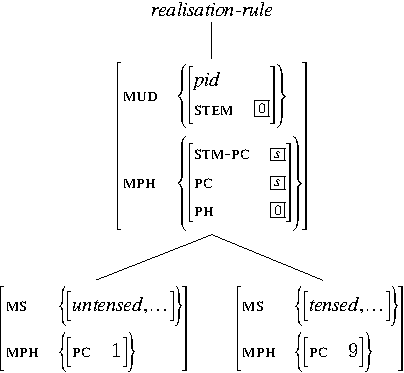
\includegraphics[scale=.9]{figures/italian-stem-crop}
  
  \caption{Partial hierarchy of Italian stem realisation rules}
  \label{fig:ItalianStem}
\end{figure}

\begin{figure}[htb]
  \centering
  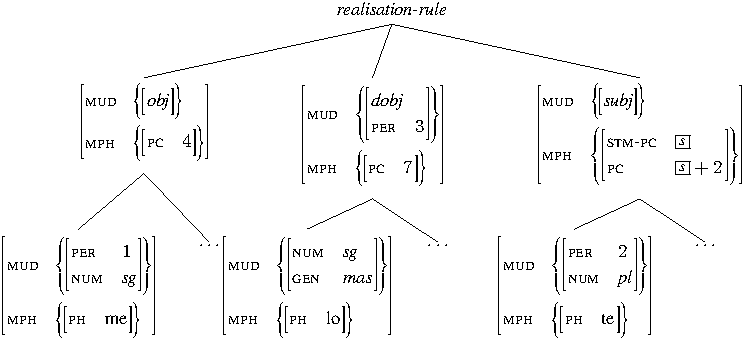
\includegraphics[scale=.84]{figures/italian-affix-crop}
  
  \caption{Partial hierarchy of Italian affixal realisation rules}
  \label{fig:ItalianAff}
\end{figure}



Compared to layered structure, the pivot feature approach appears to
be more versatile, since it provides a suitable solution to second
position affixes. In Sorani Kurdish \citep{Samvelian07}, an endoclitic agreement marker
surfaces after the initial morph, be it the stem, or some prefixal
marker. Thus, placement is relative to what ever happens to be the
first instantiated position index. 

\begin{table}
\begin{center}
{\small
\begin{tabular}[t]{lllll}
\toprule
$1$ & $2$ & $3$ & $4$\\
%\textsc{neg} & \textsc{ipfv} & send & \textsc{3pl}\\   
\midrule
    &      & nard=\textbf{jân} & im & {`they sent me'}\\
na=\textbf{jân}     &  & nard & im & {`they did not send me'}\\
    & da=\textbf{jân} & nard & im & {`they were sending me'}\\
na=\textbf{jân}     &  da  & nard & im & {`they were not sending me'}\\
\bottomrule
\end{tabular}
}
\end{center}
\caption{Sorani Kurdish past person markers\label{table-kurdish}}
\end{table}

\citet{bonami_o-crysmann_b13hpsg} propose a pivot feature \textsc{1st-pc} that is
instantiated to the position class index of the first element on the
word's \textsc{mph} list and exposed on all other morphs by the
principle in (\ref{ex:stem-principle}).

\begin{exe}
  \ex\label{ex:stem-principle}
  \begin{avm}
    {\normalfont \textit{word}\/}$\rightarrow$
    \[infl & \[mph & \<\[pc & \@1\\
        1st-pc & \@1\\stm-pc & \@s \] ,
      \[1st-pc & \@1\\
        stm-pc & \@s\] ,
    \ldots{} ,
    \[1st-pc & \@1\\stm-pc &  \@s\]
    \>
    \]\]
  \end{avm}
\end{exe}

The realisation rule for a second position clitic will then look as
follows, determining its \textsc{pc} value relative to that of the
word's first morph. I use an arithmetic operator here as a convenient
shortcut, but note that indices are actually represented as lists 
underlyingly \citep{bonami-crysmann:2013}. 

\begin{exe}
  \ex
  \begin{avm}
    \[mud & \{ \[per & 3\\
        num & pl \]\}\\
      mph & \< \[ph & <\normalfont jân>\\
        1st-pc & \@1\\
      pc & \@1 $+ 1$\]\>\]
  \end{avm}
\end{exe}

To conclude the section, a more general remark is in order: as we have
seen, IbM uses explicit position indices to constrain morphotactic
position. In essence, these correspond to linear distribution classes,
where higher indices are realised towards the right of lower indices
and no two morphs within a word may bear the same index, yielding
competition for linear position. As a consequence, there is no static
notion of a slot: while morphs are ordered according to indices, there
is no requirement for indices to be consecutive. Thus, nothing much
needs to be said about empty slots, except that there happens to be no
morph in the word with that particular positional index. 


\subsection{Constructional vs. generative views}
\label{sec:ConstrGen}

IbM departs from previous purely word-based approaches, such as
\citet{Blevins14} or, within HPSG, \citet{Koenig99} by recognising an
intermediate level of realisation rules that effects the actual $m:n$
relations between form and function. In this section, I shall discuss
how this facilitates partial generalisations over gestalt exponence,
provides for a better reuse of resources, as witnessed by parallel
inflection, and finally ensures a modular organisation of rules of
exponence.

\subsubsection{Gestalt exponence}

One of the strongest arguments for the word-based view and against a
generative rule-based approach comes from so-called gestalt exponence
in Estonian \citep{Blevins05}. As shown in Table~\ref{tab:Estonian},
core cases in this language give rise to case/number paradigms where
(almost) all cells are properly distinguished by clearly segmentable
markers, yet there is no straightforward association between the
markers and the properties they express.   


\begin{table}[htbp]
%  \centering
  \small
  \setlength{\tabcolsep}{.7\tabcolsep}
\begin{tabular}{lll}
 \multicolumn{3}{c}{\textsc{nokk} `beak'} \\
\toprule
  & \textsc{sg} & \textsc{pl}  \\
  \midrule
  \textsc{nom} & nokk & nok-a-d \\
  \textsc{gen} & nok-a & nokk-a-de\\
  \textsc{part} & nokk-a & nokk-a-sid\\
\bottomrule
\end{tabular}
\medskip
\begin{tabular}{lll} 
\multicolumn{3}{c}{\textsc{õpik} `workbook'}\\
\toprule
  & \textsc{sg} & \textsc{pl}  \\
  \midrule
  \textsc{nom}  & õpik & õpik-u-d\\
  \textsc{gen}  & õpik-u & õpik-u-te\\
  \textsc{part} & õpik-u-t & õpik-u-id \\
\bottomrule
\end{tabular}

\begin{tabular}{lll} 
\multicolumn{3}{c}{\textsc{seminar} `seminar'}\\
\toprule
  & \textsc{sg} & \textsc{pl}\\
  \midrule
  \textsc{nom}  & seminar & seminar-i-d\\
  \textsc{gen}  & seminar-i & seminar-i-de\\
  \textsc{part} & seminar-i & seminar-i-sid \\
\bottomrule
\end{tabular}
\hfill
  \caption{Partial paradigms exemplifying three Estonian noun declensions (core cases; \citealp{Blevins05})}
\label{tab:Estonian}
\end{table}

The gestalt nature of Estonian case/number marking can be schematised
as in Figure~\ref{fig:Matthews}. 

\begin{figure}[htb]
  \centering
  \begin{tabular}{lcc}
    \rnode{u1}{\textsc{beak}} & \rnode{u2}{\textsc{gen}} & \rnode{u3}{\textsc{pl}}\\[2ex]
    \rnode{l1}{nokk} & \rnode{l2}{-a} & \rnode{l3}{-de}
  \end{tabular}
      \psset{angleA=-90,angleB=90,arm=0pt,linewidth=.5pt}

      \ncdiag{u1}{l1} \ncdiag{u1}{l2} \ncdiag{u2}{l1} \ncdiag{u2}{l3}
      \ncdiag{u3}{l1} \ncdiag{u3}{l2} \ncdiag{u3}{l3}

      \caption{\emph{m}:\emph{n} relations in Estonian}
      \label{fig:Matthews}
\end{figure}

While it is clear that this kind of complex association between form
and function requires a constructional perspective, but it is far from
clear that i. this association has to be made at the top-level and
ii. that this requires word-to-word correspondences in the sense of
\citet{Blevins05,Blevins14}. To the contrary, the system depicted in
Table~\ref{tab:Estonian} displays partial generalisations that are
hard to capture in a system such as Blevins': e.g. theme vowels are
found in all cells except the nominative singular, only the nominative
singular is monomorphic, all plural forms are tri-morphic, to name
just a few.  

In IbM, $m:n$ correspondences are established at the level of
realisation rules, and it is realisation rule which are organised into
(cross-classifying) type
hierarchies. \citet{Crysmann:Bonami:2017:HPSG} argue that this
makes it possible to extract the kind of partial generalisation noted
in the previous paragraph and represent them in a three-dimensional
type hierarchy that specifies constraints on stem selection
independently of theme-vowel introduction and suffixation. Using
pre-typing, idiosyncratic aspects can be contained, while more regular
aspects, such as theme vowel and stem selection are taken care of by
Online Type Construction. 

Furthermore, encapsulating gestalt exponence as a subsystem of
realisation rules has the added advantage that it does not spill over
into the rest of the Estonian inflection system, which, as a
Finno-Ugric language,  is highly agglutinative.


While it is straightforward to implement constructional analyses
within IbM, involving complex $m:n$ relations between form and
function, non-constructional analyses are actually preferred whenever
possible, generally yielding much more parsomonious descriptions.

\subsubsection{Reuse of resources}

Cases of reuse of resources constitute a particularly strong case
against over-generalising to the constructional view: parallel
position classes are a case at hand, as exemplified in Swahili
\citep{Stump93,Crysmann:Bonami:2016} or Choc"-taw \citep{broadwell:2017}. 

\begin{table}[hbt]
  \centering
  \small
  \begin{tabular}{llllllllll}
    \toprule
    \textsc{per} & \textsc{gen} & \multicolumn{2}{l}{\textsc{subject}} &
                                                                         \multicolumn{2}{l}{\textsc{object}}\\% & \multicolumn{2}{l}{\textsc{relative}}\\
                 & & \textsc{sg} & \textsc{pl} & \textsc{sg} & \textsc{pl}\\%  & \textsc{sg} & \textsc{pl}\\
    \midrule
    1	&       & ni & tu  & ni & tu\\%  &  \\
    2	&       & u	 & m   & ku & wa\\%   \\   
    3	& \textsc{m/wa}  & a	 & wa  & m  & wa\\%   & ye & o\\
                 & \textsc{m/mi}	& u  & i   & u  & i \\%  & o & yo \\
                 & \textsc{ki/vi}	& ki & vi  & ki & vi \\% & cho & vyo \\
                 & \textsc{ji/ma} & li & ya  & li & ya \\%  & lo & yo\\
                 & \textsc{n/n} & i    & zi  & i  & zi \\%  & yo & zo\\
                 & \textsc{u}     & u  & --- & u  & --- \\% & o & ---\\
                 & \textsc{u/n}   & u  & zi  & u  & zi  \\% & o & zo\\
                 & \textsc{ku}    & ku & --- & ku & --- \\% & ko & ---\\
    \bottomrule
\end{tabular}
  \caption{Swahili person markers \citep{Stump93}} \label{ex:SwaPer} 

\end{table}

Consider the paradigms of Swahili subject and object agreement markers
in Table~\ref{ex:SwaPer}: as one can easily establish, agreement
markers draw largely on the same set of shapes. Grammatical function
is disambiguated mainly by position, with subject agreement placed 
to the left of tense markers, and object agreement to the right. 

Under a constructional approach, such as the word-based analysis in
\citet{Koenig99}, the generalisation about identity of shapes is
essentially lost: this is due to the fact that under this view,
markers that can potentially combine must be introduced in different
cross-classifying dimensions, e.g. one for subject marking in slot 2,
the other for object marking in slot 5. Likewise, in order to
distribute shape constraints over subject and object agreement, they
must constitute yet another cross-cutting dimension, but there is
simply no way in this set-up to enforce that every shape constraint
must be evaluated twice.  

\begin{figure*}[htb]
  \centering
  \smaller\smaller
\begin{forest}
[\emph{realisation-rule}
	[SHAPE,draw
		[{\begin{avm}
			\[ mph & \{\[ph &  \<\normalfont ni\>\]\}\\
			mud & \{\[per & 1\\ num & sg\]\}
			\]
		\end{avm}}, name=1
			[{\begin{avm}
				\[ mph & \{\[ph &  \<\normalfont ni\>\\ pc & 2\]\}\\
				mud & \{ \[\asort{subj} per & 1\\ num & sg\] \}
				\]
			\end{avm}}, name=a, no edge, tier=word, l=3cm]
		]
		[{\begin{avm}
			\[ mph & \{\[ph &  \<\normalfont wa\>\]\}\\
			mud & \{\[per & 3\\ num & pl\]\}
			\]
		\end{avm}}, name=2
			[{\begin{avm}
				\[ mph & \{\[ph &  \<\normalfont wa\>\\ pc & 5\]\}\\
				mud & \{ \[\asort{obj} per & 3\\ num & pl\] \}
				\]
			\end{avm}}, name=b, no edge, tier=word, l=3cm]
		]
	]
	[POSITION,draw
		[{\begin{avm}
			\[ mph & \{\[pc & 2\]\}\\
			mud & \{subj\}
			\]
		\end{avm}}, name=3
			[{\begin{avm}
				\[ mph & \{\[ph &  \<\normalfont wa\>\\ pc & 2\]\}\\
				mud & \{ \[\asort{subj} per & 3\\ num & pl\] \}
				\]
			\end{avm}}, name=c, no edge, tier=word, l=3cm]
		]
		[{\begin{avm}
			\[ mph & \{\[pc & 5\]\}\\
			mud & \{ obj \}
			\]
		\end{avm}}, name=4
			[{\begin{avm}
				\[ mph & \{\[ph &  \<\normalfont ni\>\\ pc & 5\]\}\\
				mud & \{\[\asort{obj} per & 1\\ num & sg\]\}
				\]
			\end{avm}}, name=d, no edge, tier=word, l=3cm]
		]
	]
]
\draw[dashed] (1.south) to (a.north);
\draw[dashed] (1.south) to (d.north);
\draw[dashed] (2.south) to (b.north);
\draw[dashed] (2.south) to (c.north);
\draw[dashed] (3.south) to (c.north);
\draw[dashed] (3.south) to (a.north);
\draw[dashed] (4.south) to (b.north);
\draw[dashed] (4.south) to (d.north);
\end{forest}
  
  \caption{Rule type hierarchy for Swahili parallel position classes \citep{Crysmann:Bonami:2016}}
  \label{fig:Swahili}
\end{figure*}

However, once we move from word-based statements to realisation rules,
the problem simply vanishes, since we are not trying to solve the
problem of parallel inflection and combinbation at the same time: as
illustrated in Figure~\ref{fig:Swahili}, constraints about shape can
be straightforwardly distributed over realisation rules for subject
and object agreement (which are types), because their combination is
effectively factored out. Thus, by abstracting over rules instead of
words, generalisation about parallel inflection can be captured quite
easily. This is in fact a more general problem that tends to get
overlooked by radically word-based approaches such as
\citet{Blevins14}.

\subsubsection{Modularity}

The final argument for combining constructional or holistic with
generative or atomistic views is that it provides for a divide and
conquer approach to complex inflectional systems.

\citet{diaz:koenig:michelson:19} discuss the pre-pronominal affix
cluster in Oneida, an Iroquoian language. Oneida presents us with what
is probably the most complex morphotactic system that has been
described so far within IbM.

Oneida is a highly poly-synthetic language. According to
\citet{diaz:koenig:michelson:19}, the inflectional system alone
comprises seven prefixal position classes in which up to eight
non-modal and three modal categories can be expressed
(cf. Table~\ref{tab:Oneida}). Given the number of categories and
position alone, it comes at no surprise that the system is
characterised by heavy competition. Adding to the complexity, several
markers undergo complex interactions, even between non-adjacent slots.
Finally, Oneida pre-pronominal prefixes also display variable
morphotactics: e.g. the factual appears in four different surface
positions, and the optative in three. Moreover, we find paradigmatic
misalignment (cf. the discussion of Nepali above), with the
cislocative in a different surface position from the translocative.

\begin{table}[htb]
  \centering
  \scriptsize
  \begin{tabular}{l|l|l|l|l|l|l|l}
    \toprule
    1&2&3&4&5&6&7&8\\
    \midrule    Negative & Translocative & Dualic & Factual & Cislocative &
                                                                Factual
               & Pronominal & Stem\\

    Contrastive & Factual & & Optative & Repetitive & Optative &
                                                                 Factual
                 & \\
    Coincident & & Future & & Optative & &  \\
    Partitive & & & & & & &\\
    \bottomrule
  \end{tabular}
  \caption{Position classes of Oneida inflectional prefixes}
  \label{tab:Oneida}
\end{table}

\citet{diaz:koenig:michelson:19} discuss three different types of
interaction within the system: (i) positional competition, exhibited
in slot 1 (negative, contrastive, coincidental, partitive) and slot 5
(cislocative, repetitive); (ii) borrowing, a particular case of extended
exponence exhibited in slot 2 (translocative borrowing vowels from the
future and factual); and (iii) sharing, witnessed by the factual and
the optative, which are distributed across different positions. Cross-cutting these subsystems, we find a great level of
contextual inflectional allomorphy.

\citet{diaz:koenig:michelson:19} contain the complexity of the system
by building on several key notions, the first three of
which are integral parts of IbM: first, the fact that IbM recognises
$m:n$ relations at the rule level make it possible to approach the
Oneida system in a more modular fashion carving out four independent
subsystems for competition (slot 1 and slot 5), borrowing (slot 2) and
sharing (factual). Second, they draw on the distinction between
realisation (\textsc{mud}) and conditioning \textsc{ms} to abstract
out inflectional allomorphy. Third, they capture discontinuous
exponence of the factual and optative in terms of Koenig/Jurafsky
style cross-classification in order to derive complex discontinuous
rules.

The two innovative aspects of their analysis concern the treatment of
competition and an abstraction over morpho-syntactic properties in
terms of syntagmatic classes. Oneida resolves morphotactic competition
of semantically compatible features (slots 1 and 5) by means of a
markedness hierarchy: features that are outranked on this hierarchy
are optionally interpreted if the exponent of a higher feature is
present. E.g. the negative outranks the partitive, so if the negative
marker is present, it can be interpreted as negative or negative and
partitive. If, by contrast, the partitive marker is found, the
negative cannot be understood.  \citet{diaz:koenig:michelson:19}
approach this by modelling the ranking in terms of a type hierarchy
upon which realisation rules can draw. Their second innovation, i.e. 
the  segregation of morpho-semantic properties according to
the positional properties of their exponents into e.g. inner or outer
types has enabled them to give a much more concise representation of
allomorphy that can abstract over strata of positions. 

The combination of design properties of IbM with their two innovations
have permitted \citet{diaz:koenig:michelson:19} to provide an explicit
and surprisingly concise analysis of an extremely complex system: in
essence, their highly modular analysis (with only 36 rules) reduces the
number of allomorphs by a factor of ten.

\bigskip\noindent In sum, having $m:n$ relations at the most basic
level of realisation rules means that constructional views can be
implemented at any level of granularity, combining reuse and
recombination, as favoured by an atomistic (generative) view, with the
holistic (constructional) view necessitated by discontinuous or
gestalt exponence.  To quote \citet{diaz:koenig:michelson:19}, ``IbM’s
approach to morphology [...] is something unification-based approaches
to syntax have stressed for the last forty-years or so'': in addition
to the model-theoretic aspect they capitalise on, the similarity of
IbM to current HPSG syntax also pertains to the fact that both integrate
lexicalist and constructional views.

\section{Conclusion}

This chapter has provided an overview of HPSG work in two core areas
of morphology, namely derivation and inflection. The focus of this
paper was biased to some degree towards inflection, for two reasons:
on the one hand, a handbook article that provides a more balanced
representation of derivational and inflectional work in
constraint-based grammar was published quite recently
\citep{Bonami15b}, while on the other, a comprehensive introduction
to recent development within HPSG inflectional morphology was still
missing.

In the area of derivation and grammatical function change, a consensus
has been reached relatively early, toward the end of the last century,
with the works of \citet{Riehemann98} and \cite{Koenig99}:
within HPSG, it is now clearly understood that lexical rules are
description level devices organised into cross-cutting inheritance
type hierarchies. Beyond HPSG these works have influenced the
development of Construction Morphology \citep{Booij10}, cf.\ also
Chapter ~\crossrefchaptert{cxg}. 

Much more recently, some consensus model seems to have arrived for the
treatment of inflectional morphology: Information-based Morphology
\citep{Crysmann:Bonami:2016,Crysmann:14:OUP} build on previous work on
inflectional morphology in HPSG (Bonami), Online Type Construction
\citep{Koenig99}, morph-based morphology \citep{crysmann_b03book}, and
finally unification-based approaches to Pāṇini's principle
\citep{Andrews90,Erjavec94,Koenig99} to provide an
inferential-realisational theory of morphology that exploits the same
logic as HPSG, namely typed feature structure inheritance network to
capture linguistic generalisations. Furthermore, like its syntactic
parent, it permits to strike a balance between lexicalist and
constructional views.





\printbibliography[heading=subbibliography,notkeyword=this]

\end{document}


%%% Local Variables:
%%% mode: latex
%%% TeX-master: "../main-udc"
%%% End:
